\chapter{Nonlinear model predictive control for steerable WMRs}
\label{ch:nmpc-swmr}
Steerable wheeled mobile robots (SWMRs) are known to be flexibile and robust
thanks to their omnidirectionality and the presence of conventional wheels.
Nevertheless, their modeling and control is complex, due
to the presence of singularities in their representation or in the control
scheme.

In this chapter, we consider the problem of trajectory tracking for steerable
wheeled mobile robots (SWMRs), equipped with two or more wheels.
The robot is required to follow a user-defined reference pose trajectory in
an environment free of obstacles, without violating the driving and steering
velocity constraints of each wheel. Note that, in order to successfully perform
this task, it is of utmost importance to take into account the kinematic
singularities of the platform \cite{Sorour2019RAS}. To solve this
problem, we propose a framework which makes use of
Nonlinear Model Predictive Control \cite{Rawlings2017MPCBook}.
While many existing work use MPC on differential drive robots \cite{Tarantos2023Springer},
on autonomous vehicles such as cars \cite{Zanon2014Springer} and tractor trailers
\cite{Beglini2022TMECH}, and on wheeled-legged robots \cite{Bjelonic2021IROS},
the application of MPC to SWMRs has yet to be explored.

\begin{figure}
    \centering
    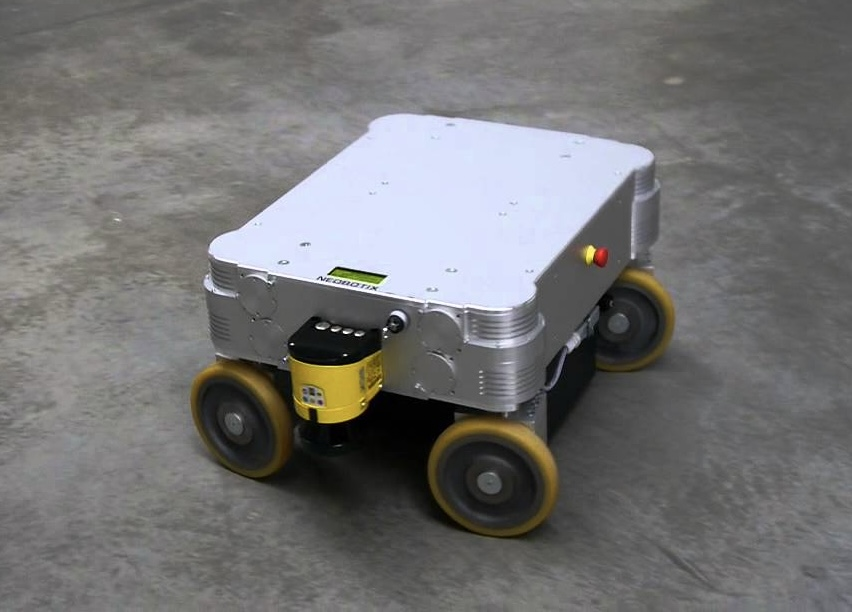
\includegraphics[width=0.7\textwidth]{figures/SWMR/mpo-700.jpg}
    \caption{The Neobotix MPO-700 steerable wheeled mobile robot.}
    \label{fig:mpo-700}
\end{figure}

Our NMPC is supported by a \textit{finite state machine}, responsible for
starting and stopping the motion of the robot, while guaranteeing that it never
encounters any kinematic singularity, and
a \textit{state trajectory generation scheme} based on dynamic
feedback linearization \cite{Oriolo2002WMRControlDFL}, which generates
reference configurations and reference control inputs for the NMPC
itself, given the reference pose trajectory. 
The NMPC is formulated as a Nonlinear Programming problem, and solved using the
real-time iteration scheme \cite{Gros2020Fromlineartononlinear}.
Our approach is validated on a
Neobotix MPO-700 on trajectories of increasing difficulty.

\section{Kinematic model}
\label{sec:kinematic-model}
In this section, we will develop the kinematic model of a steerable wheeled
mobile robot (SWMR), following the analysis presented in
\cite{RobuffoGiordano2009ICRA}. Note that while our mobile base is equipped
with steerable wheels, its kinematic model is identical to the one described
in \cite{RobuffoGiordano2009ICRA}, which considers caster wheels.

Consider a SWMR equipped with $n_s \ge 2$ independent steerable wheels.
With reference to Fig. \ref{fig:swmr}, we will denote the vector
$\bm{\xi} = [x, y, \theta]^\top \in SE(2)$ as the pose of mobile base,
with $(x, y)$ its position and $\theta$ its orientation. Let $S_i$ be
the $i$-th steering joint of the mobile base, and $W_i$ the $i$-th wheel of
the mobile base, and let $\bm{o}_{S_i}$ and $\bm{o}_{W_i}$ respectively be
their positions, the latter parameterized by the steering angle $\beta_i$.
Each wheel is also described by two independent velocities, the driving
velocity $v_{Wi}$ and the steering velocity $v_{\beta_i}$, which are taken
as control inputs. We define the whole robot configuration via the vector
$\bm{q}=[\bm{\xi}^\top, \bm{\beta}^\top]^\top$, where
$\bm{\beta}=[\beta_1, \dots, \beta_{n_s}]^\top$.

\begin{figure}
    \centering
    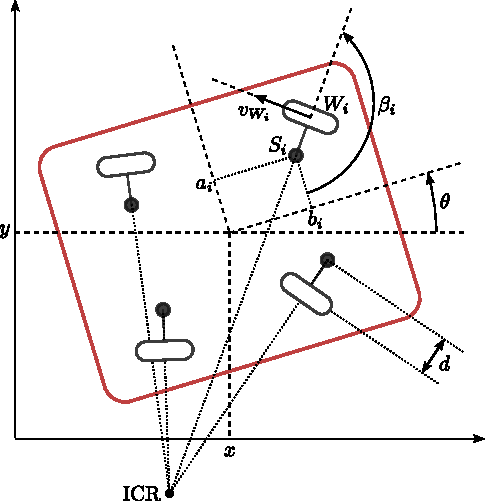
\includegraphics[width=0.65\textwidth]{figures/SWMR/swmr.pdf}
    \caption{Schematic model of a SWMR. Note that, even if the figure
        represents a robot equipped with four wheels, our approach is generic
        and works with an arbitrary number of 2 or more wheels.}
    \label{fig:swmr}
\end{figure}

The position of the $i$-th steering joint $S_i$ is defined as
\begin{align*}
    \bm{o}_{S_i} &=
    \begin{bmatrix}
        x \\
        y
    \end{bmatrix}
    +
    \bm{R}(\theta)
    \begin{bmatrix}
        b_i \\
        a_i
    \end{bmatrix},
\end{align*}
and the position of the $i$-th wheel $W_i$ is defined as
\begin{align*}
    \bm{o}_{W_i} &=
    \bm{o}_{S_i}
    +
    \bm{R}(\theta + \beta_i)
    \begin{bmatrix}
        0 \\
        -d
    \end{bmatrix}.
    %\\&=
    %\begin{bmatrix}
    %    x + b_i \cos\theta - a_i \sin\theta + d \sin(\theta + \beta_i) \\
    %    y + b_i \sin\theta + a_i \cos\theta - d \cos(\theta + \beta_i),
    %\end{bmatrix}
\end{align*}
where $\bm{R} \in SO(2)$ is a rotation matrix.
%while its velocity can be defined by
%\begin{align*} 
%    \dot{\bm{o}}_{W_i} &=
%    \begin{bmatrix}
%        \dot{x} \\
%        \dot{y}
%    \end{bmatrix}
%    +
%    \dot{\bm{R}}(\theta)
%    \begin{bmatrix}
%        b_i \\
%        a_i
%    \end{bmatrix}
%    +
%    \dot{\bm{R}}(\theta + \beta_i)
%    \begin{bmatrix}
%        0 \\
%        -d
%    \end{bmatrix}
%    \\&=
%    \begin{bmatrix}
%        \dot{x} - (b_i \sin\theta + a_i \cos\theta) \dot{\theta} + d \cos(\theta + \beta_i) (\dot{\theta} + \dot{\beta}_i) \\
%        \dot{y} + (b_i \cos\theta - a_i \sin\theta) \dot{\theta} + d \sin(\theta + \beta_i) (\dot{\theta} + \dot{\beta}_i)
%    \end{bmatrix}.
%\end{align*}

Due to the assumption of no lateral skidding (i.e., the velocity of the contact
point of the wheel must be orthogonal with respect to the zero motion line of
the wheel itself), each wheel is subject to the Pfaffian constraint
\begin{equation}
    \label{eq:no-lateral-skidding-constraint}
    \begin{bmatrix}
        -\sin(\theta + \beta_i) \\
         \cos(\theta + \beta_i)
    \end{bmatrix}^\top \dot{\bm{o}}_{W_i} = 0.
\end{equation}
%which can be rewritten as
%\begin{equation}
%    \label{eq:no-lateral-skidding-constraint}
%    -\sin(\theta + \beta_i) \dot{x} +
%    \cos(\theta + \beta_i) \dot{y} +
%    (b_i \cos(\beta_i) + a_i \sin(\beta_i)) \dot{\theta} = 0.
%\end{equation}

By combining the above equations, it is possible to rearrange the $n_s$ constraints in matrix form
\begin{equation}
    \label{eq:pfaffian-constraints-matrix-form}
    \underbrace{
    \begin{bmatrix}
        -\sin(\theta + \beta_1) &
        \cos(\theta + \beta_1) &
        \Delta_1 &
        0 \dots 0 \\
        -\sin(\theta + \beta_2) &
        \cos(\theta + \beta_2) &
        \Delta_2 &
        0 \dots 0 \\
        \vdots & \vdots & \vdots & \vdots \\
        -\sin(\theta + \beta_{n_s}) &
        \cos(\theta + \beta_{n_s}) &
        \Delta_{n_s} &
        0 \dots 0 \\
    \end{bmatrix}
    }_{\bm{A}^\top(\bm{q})}
    \dot{\bm{q}} = 0,
\end{equation}
with $\Delta_i = b_i \cos\beta_i + a_i \sin\beta_i$.

For the mobile base to perform a motion, all wheel axles must instantaneously
intersect at the same point, the ICR. The existence of an ICR can also be seen
as a geometric constraint, which requires all wheel orientations to be
coordinated. In the following, we will study how the ICR constraint affects
the robot mobility.

\subsection{ICR constraint not satisfied}
Whenever the robot configuration is such that it has no instantaneous center
of rotation (ICR), since from~(\ref{eq:pfaffian-constraints-matrix-form})
$\dot{\bm{q}} \in \mathcal{N}(\bm{A}^\top(\bm{q}))$, the kinematic model of
the robot is the following:
\begin{align*}
\begin{split}
%    \dot{x} &= 0 \\
%    \dot{y} &= 0 \\
%    \dot{\theta} &= 0 \\
    \dot{\beta}_i &= v_{\beta_i},
\end{split}
\end{align*}
with $v_{\beta_i}$ steering velocities. In this case, the pose of the robot
remains constant, and it is only possible to control the steering angles. 

\subsection{ICR constraint satisfied}
\label{sec:icr-constraint-satisfied}
Whenever the robot configuration is such that there exists an ICR,
it is possible to simplify~\eqref{eq:pfaffian-constraints-matrix-form}
through the use of \textit{coordinating functions} for $\beta_i$
\cite{RobuffoGiordano2009ICRA}, with $i \ge 2$. The idea is to let the ICR
be defined by the trajectory of $\bm{\xi}$, namely $\bm{\xi} \left( t \right)$.
Indeed, considering the $i$-th constraint in
\eqref{eq:pfaffian-constraints-matrix-form} and solving for $\beta_i$ yields
the coordinating function\footnote{Note that $\beta_i$ can have two values,
shifted by $\pi$. We select the one closest to the current $\beta_i$.}
(holonomic constraint)
\begin{equation}
    \label{eq:coordinating-function-pre-kinematic-model}
    \beta_i = h_i(\bm{\xi}, \dot{\bm{\xi}}) = \mathrm{arctan} \frac{-\sin\theta\dot{x}+\cos\theta\dot{y}+b_i\dot{\theta}}{\cos\theta\dot{x}+\sin\theta\dot{y}-a_i\dot{\theta}},
\end{equation}
which can be used to transform the last $n_s-1$ constraints of
\eqref{eq:pfaffian-constraints-matrix-form}, obtaining:
\begin{equation}
    \label{eq:reduced-pfaffian-constraints-matrix-form}
    \begin{bmatrix}
        -\sin(\theta + \beta_1) &
        \cos(\theta + \beta_1) &
        \Delta_1 &
        0
    \end{bmatrix}
    \begin{bmatrix}
        \dot{x} \\ \dot{y} \\ \dot{\theta} \\ \dot{\beta}_1
    \end{bmatrix}
    = 0,
\end{equation}
\begin{equation*}
    \beta_i = h_i(\bm{\xi}, \dot{\bm{\xi}}), \quad i = 2, \dots, n_s.
\end{equation*}

From \eqref{eq:reduced-pfaffian-constraints-matrix-form}, it is trivial to
get the reduced kinematic model
\begin{equation}
\label{eq:reduced-kinematic-model}
\begin{split}
    \dot{x} &= v_{S_1} \cos(\theta + \beta_1) + \omega (b_1 \sin\theta + a_1 \cos\theta) \\
    \dot{y} &= v_{S_1} \sin(\theta + \beta_1) + \omega (-b_1 \cos\theta + a_1 \sin\theta) \\
    \dot{\theta} &= \omega \\
    \dot{\beta}_1 &= v_{\beta_1},
\end{split}
\end{equation}
which can be used together with \eqref{eq:coordinating-function-pre-kinematic-model}
to express $\beta_i$ as
\begin{equation}
    \label{eq:coordinating-function-post-kinematic-model}
    \beta_i = h_i(v_{S_1}, \omega, \beta_1) = \mathrm{arctan} \frac{v_{S_1}\sin\beta_1+\omega(b_i-b_1)}{v_{S_1}\cos\beta_1+\omega(a_1-a_i)}.
\end{equation}

Note that the above equations (named \textit{coordinating functions}) present a singularity whenever the position of the $i$-th steering joint $S_i$ is constant (i.e., $\dot{\bm{o}}_{S_i}=\bm{0}$). This needs to be considered when designing a controller. Note that this condition is met when the platform is not moving or when the position of the ICR coincides with the position of $S_i$. 

As a consequence, if the ICR does not lie on any of the steering joints $S_i$
and if it does not change through time (i.e. $\dot{\beta}_i = 0$), all
coordinating functions $h_i$ are free of singularity. Two interesting cases when
these hypotheses hold are when the ICR is constant at infinity
(i.e., $\omega = 0$), and when the ICR is constant, not at infinity
(i.e., $v_{S_1} = \omega R$, with $R > 0$ the distance between ICR and
$\bm{o}_{S_1}$). Hereby, we define the reduced kinematic models and coordinating
functions for these 2 cases, which we use to start/stop the robot.

\begin{figure}
    \centering
    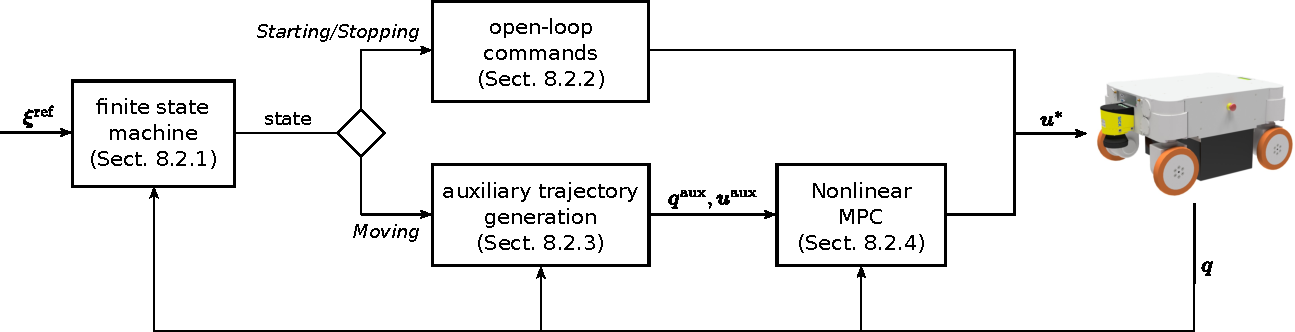
\includegraphics[width=\textwidth]{figures/SWMR/blockscheme.pdf}
    \caption{Block scheme of the proposed framework. A user-defined reference
        pose trajectory $\bm{\xi}^{\rm ref}$ is fed to a Finite State Machine (FSM),
        which determines when to start/stop robot motion. As soon as a reference
        trajectory is available, the state of the FSM becomes \textit{Starting},
        and the mobile base is accelerated (using open-loop commands) until all
        wheel driving velocities are non null. When this condition is met, the
        state of the FSM becomes \textit{Moving}, and the Nonlinear MPC takes
        full control of the robot motion. In this case, a state trajectory
        generation scheme based on dynamic feedback linearization computes the
        trajectories $\bm{q}^{\rm ref}$ and $\bm{u}^{\rm ref}$
        (using $\bm{\xi}^{\rm ref}$), which are used by the Nonlinear MPC to
        compute control inputs $\bm{v}_{W_i}, \bm{\beta}_i$.
        The state of the FSM becomes \textit{Stopping} when
        $\bm{\xi}^{\rm ref} = \bm{0}$, and the robot decelerates, then stops.
    }
    \label{fig:block-scheme}
\end{figure}

\begin{figure}
    \centering
    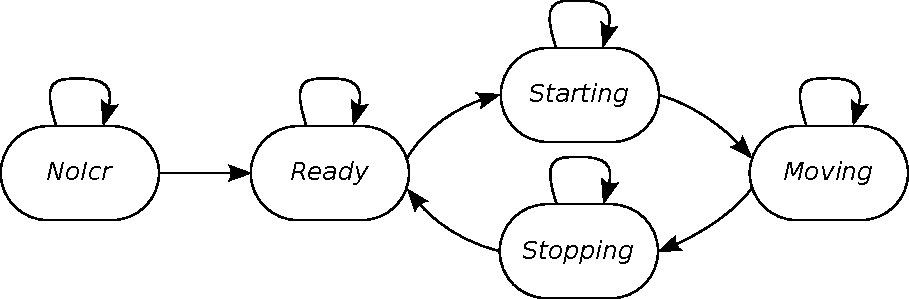
\includegraphics[width=0.7\textwidth]{figures/SWMR/finitestatemachine.pdf}
    \caption{Finite state machine defining the motion of the mobile base.}
    \label{fig:finite-state-machine}
\end{figure}


\subsubsection{ICR constant at infinity}
\label{sec:icr-constant-at-infinity}
in this case, the steering angles are the same for all wheels and $\omega = 0$.
Then, the robot's reduced kinematic model \eqref{eq:reduced-kinematic-model} becomes
\begin{align}
\label{eq:icr-constant-at-infinity-kinematic-model}
\begin{split}
    \dot{x} &= v_{S_1} \cos(\theta + \beta_1) \\
    \dot{y} &= v_{S_1} \sin(\theta + \beta_1), \\
%    \dot{\theta} &= 0 \\
%    \dot{\beta}_1 &= 0,
\end{split}
\end{align}
and the coordinating functions become
\begin{equation*}
    \beta_i = h_i(\beta_1) = \beta_1.
\end{equation*}
The robot can only move along a line parallel to the wheels' sagittal axes.

\subsubsection{ICR constant not at infinity}
\label{sec:icr-constant-not-at-infinity}
in this case, the robot's reduced kinematic model \eqref{eq:reduced-kinematic-model} becomes
\begin{align}
\label{eq:icr-constant-not-at-infinity-kinematic-model}
\begin{split}
    \dot{x} &= \omega R \cos(\theta + \beta_1) + \omega (b_1 \sin\theta + a_1 \cos\theta) \\
    \dot{y} &= \omega R \sin(\theta + \beta_1) + \omega (-b_1 \cos\theta + a_1 \sin\theta) \\
    \dot{\theta} &= \omega, \\
%    \dot{\beta}_1 &= 0,
\end{split}
\end{align}
and the coordinating functions become
\begin{equation*}
    \beta_i = h_i(\beta_1) = \mathrm{arctan}\frac{R \sin\beta_1 + b_i - b_1}{R \cos\beta_1 + a_1 - a_i}.
\end{equation*}
Note that $R$ can be determined from the ICR, which can be computed as the
intersection of the wheel axles. In this case, the robot can only move along
the circle centered at the ICR, and radius corresponding to the distance between
the position of the robot and the ICR itself.

\section{Proposed framework}
\label{sec:proposed-framework}
This section describes in detail the main components of our framework
(shown in Fig. \ref{fig:block-scheme}), namely: the finite state machine,
responsible for starting and stopping the robot while avoiding kinematic
singularities, the state trajectory generation scheme, which provides
trajectories to the NMPC, and the NMPC itself, which computes control inputs
for the robot, while satisfying the driving and steering velocity constraints
of each wheel.

\subsection{Finite state machine}
\label{sec:finite-state-machine}
Since the ICR constraint may not be satisfied at initialization, and since the
NMPC must avoid configurations in which coordinating functions
\eqref{eq:coordinating-function-post-kinematic-model} are singular, we
designed a finite state machine (FSM) to move the robot towards a configuration
free of singularity.

The FSM, shown in Fig. \ref{fig:finite-state-machine}, consists of five states,
described -- along with the triggering events -- hereby.
\begin{itemize}
    %\renewcommand{\labelitemi}{$\blacktriangleright$}
    \item[$\blacktriangleright$] \textit{NoICR}. The configuration of the robot
        is such that the ICR constraint is not satisfied. In this state, the
        wheels are regulated to a user-defined configuration using a
        proportional controller. Once the ICR constraint is satisfied,
        the state of the FSM becomes \textit{Ready}.

    \item[$\blacktriangleright$] \textit{Ready}. The configuration of the robot
        is such that the ICR constraint is satisfied and the robot is not
        moving. Once a new trajectory is available, the state of the FSM
        becomes \textit{Starting}.
    
    \item[$\blacktriangleright$] \textit{Starting}. An open loop controller
        makes the robot start its motion taking into account the
        singularity-free kinematic models previously presented: either
        \eqref{eq:icr-constant-at-infinity-kinematic-model} or
        \eqref{eq:icr-constant-not-at-infinity-kinematic-model},
        depending on the robot's initial configuration. Once all velocities
        $\dot{\bm{o}}_{S_i}$ become non-null, the state of the FSM becomes
        \textit{Moving}.
    
    \item[$\blacktriangleright$] \textit{Moving}. The robot moves using the
        NMPC. If the trajectory tracking task is about to be be completed,
        the state of the FSM becomes \textit{Stopping}.

    \item[$\blacktriangleright$] \textit{Stopping}. Similarly to
        \textit{Starting}, an open loop motion makes the mobile base reduce
        its speed until it stops. Once the robot stops its motion, the state
        of the FSM becomes \textit{Ready}.
\end{itemize}

\subsection{Open-loop commands (starting and stopping)}
\label{sec:starting-and-stopping}
In this section, we present our singularity-free strategy, for handling
starting and stopping motions. To this end, we first constrain the ICR to be
constant, as explained in Sect.~\ref{sec:icr-constraint-satisfied}, and we
accelerate (respectively, decelerate) the mobile base along the arc of circle
defined by the initial position of the robot and the initial ICR, until all
velocities $\dot{\bm{o}}_{S_i}$ are non-null (respectively, null).

If the ICR is constant at infinity, the robot evolves according
to~\eqref{eq:icr-constant-at-infinity-kinematic-model}.
Considering the dynamic extension $\dot{v}_{S_1}=a_{S_1}$, with $a_{S_1}$ new control input:
\begin{itemize}
    \item when the state of the FSM is \textit{Starting},
        we accelerate the mobile base by choosing
        $a_{S_1} = a_{S_1}^{\mathrm{init}}$, where $a_{S_1}^{\mathrm{init}}$
        is a parameter;
    \item when the state of the FSM is \textit{Stopping}, we decelerate the
        mobile base by choosing $a_{S_1} = -K_{v_{S_1}}^{\mathrm{stop}} v_{S_1}$,
        with $K_{v_{S_1}}^{\mathrm{stop}} > 0$.
\end{itemize}

Assuming that the ICR is constant, but not at infinity and not lying on any of
the steering joint, the robot evolves according to~\eqref{eq:icr-constant-not-at-infinity-kinematic-model}.
Considering the dynamic extension $\dot{\omega}=a_{\omega}$, with
$a_{\omega}$ new control input:
\begin{itemize}
    \item when the state of the FSM is \textit{Starting}, we accelerate the
        mobile base via $a_{\omega} = a_{S_1}^{\mathrm{init}} / R$, which,
        since $\dot{v}_{W_1}=a_{\omega} R$, is equivalent to accelerate $S_1$ by $a_{S_1}^{\mathrm{init}}$;
    \item when the state of the FSM is \textit{Stopping}, we decelerate the
        mobile base via $a_{\omega} = -K_{v_{S_1}}^{\mathrm{stop}} v_{S_1} / R$,
        which is equivalent to decelerate $S_1$ by $-K_{v_{S_1}}^{\mathrm{stop}} v_{S_1}$.
\end{itemize}

\subsection{State trajectory generation}
Once the velocities $\dot{\bm{o}}_{S_i}$ become non-null, the state becomes
\textit{Moving}, and the robot is controlled by the NMPC. In this section, we
present the state trajectory generation scheme based on dynamic feedback
linearization \cite{Oriolo2002WMRControlDFL}, which computes state
configurations and control input trajectories for the NMPC, given a reference
pose trajectory $\bm{\xi}^{\mathrm{ref}}$ of the mobile base. Note that both
state trajectory generation and NMPC are only active when the state is
\textit{Moving}.

Consider the output function $\bm{z}(\bm{q})=\bm{\xi}$ and dynamically extend
\eqref{eq:reduced-kinematic-model} by adding the following integrators:
\begin{subequations}
    \begin{align*}
        \dot{v}_{S_1} &= a_{S_1} \\
        \dot{\omega} &= a_{\omega},
    \end{align*}
\end{subequations}
so that $\bm{u} = \left[ a_{S_1}, a_{\omega}, v_{\beta_1} \right]^\top $ are
the new control inputs. In the following, unless otherwise specified, we denote
the robot configuration with dynamic extension as
$\bm{q} = [x, y, \theta, \beta_1, v_{S_1}, \omega]^\top$.
%Note that $\bm{q}$ is a non-minimal configuration.
The dynamically extended kinematic model is
\begin{equation}
\label{eq:dynamically-extended-kinematic-model}
\begin{split}
    \dot{x} &= v_{S_1} \cos(\theta + \beta_1) + \omega (b_1 \sin\theta + a_1 \cos\theta) \\
    \dot{y} &= v_{S_1} \sin(\theta + \beta_1) + \omega (-b_1 \cos\theta + a_1 \sin\theta) \\
    \dot{\theta} &= \omega \\
    \dot{\beta}_1 &= v_{\beta_1} \\
    %\dot{\beta}_i &= \dot{h}_i(\bm{q}, \bm{u}), \quad i = 2, \dots, n_s \\
    \dot{v}_{S_1} &= a_{{S_1}} \\
    \dot{\omega} &= a_{\omega},
\end{split}
\end{equation}
which, in the following, will be denoted as $\dot{\bm{q}} = \bm{f}(\bm{q}, \bm{u})$.

By deriving twice $\bm{z}(\bm{q})$, we obtain
\begin{equation}
\label{eq:zddot}
    \ddot{\bm{z}}(\bm{q})
    =
    \begin{bmatrix}
        \ddot{x} \\ \ddot{y} \\ \ddot{\theta}
    \end{bmatrix}
    =
    \bm{M}(\bm{q}) +
    \bm{H}(\bm{q})
    \begin{bmatrix}
        a_{S_1} \\ a_{\omega} \\ v_{\beta_1}
    \end{bmatrix},
\end{equation}
with $\bm{M}(\bm{q}) \in \mathbb{R}^3$ and $\bm{H}(\bm{q}) \in \mathbb{R}^{3 \times 3}$ defined as
\begin{align*}
    \bm{M}(\bm{q})
    &=
    \begin{bmatrix}
        -\sin(\theta+\beta_1) \omega v_{S_1} + ( b_1 \cos\theta - a_1 \sin\theta) \omega^2 \\
         \cos(\theta+\beta_1) \omega v_{S_1} + (-b_1 \sin\theta + a_1 \cos\theta) \omega^2 \\
        0
    \end{bmatrix}, \\
    \bm{H}(\bm{q})
    &=
    \begin{bmatrix}
        \cos(\theta+\beta_1) &  b_1 \sin\theta + a_1 \cos\theta & -\sin(\theta+\beta_1) v_{S_1} \\
        \sin(\theta+\beta_1) & -b_1 \cos\theta + a_1 \sin\theta &  \cos(\theta+\beta_1) v_{S_1} \\
        0 & 1 & 0
    \end{bmatrix}.
\end{align*}

By choosing
\begin{equation*}
    \bm{u} = \begin{bmatrix}
        a_{S_1} \\ a_{\omega} \\ v_{\beta_1}
    \end{bmatrix}
    = \bm{H}(\bm{q})^{-1} \left(\bm{a} - \bm{M}(\bm{q})\right),
\end{equation*}
we can transform~\eqref{eq:zddot} into an equivalent chain of integrators
\begin{equation*}
    \ddot{\bm{z}} = \bm{a},
\end{equation*}
which can be easily stabilized. Indeed, exponential regulation of the trajectory
tracking error $\bm{e}(t) = \bm{z}^{\mathrm{ref}}(t)-\bm{z}(t)$, can be
achieved by taking
\begin{equation*}
    \bm{a} = \ddot{\bm{z}}^{\mathrm{ref}} + \bm{K}_P \bm{e} + \bm{K}_D \dot{\bm{e}}, \quad \bm{K}_P, \bm{K}_D > 0,
\end{equation*}
with $\bm{z}^{\mathrm{ref}}(t)$ twice differentiable and persistent
(i.e., $v_{S_1} \ne 0$) reference trajectory. Note that the above decoupling
matrix $\bm{H}(\bm{q})$ is singular at $v_{S_1} = 0$. This kind of singularity
is structural for mobile robots \cite{Oriolo2002WMRControlDFL}.

Given the reference trajectories
$\bm{\xi}^{\mathrm{ref}}, \dot{\bm{\xi}}^{\mathrm{ref}}, \ddot{\bm{\xi}}^{\mathrm{ref}}$,
Algorithm \ref{alg:StateTrajectoryGeneration} generates, at each timestep
$t_k$, the states $\bm{q}_{j|k}^{\mathrm{ref}}$ ($j = 0, \dots, N$),
together with the control inputs
$\bm{u}_{j|k}^{\mathrm{ref}}$ ($j = 0, \dots, N-1$). These will be used by the
NMPC, described in the next section, to compute control inputs
$(a_{S_1, k}, a_{\omega, k}, v_{\beta_1, k})^T$ for the mobile base.
In the pseudocode: function $\mathrm{Sample}$ discretizes a trajectory,
given over a time interval $[t_k, t_{k} + N \delta_{\mathrm{MPC}}]$, into
$N + 1$ elements, with $\delta_{\mathrm{MPC}}$ timestep of the NMPC, and
function $\bm{F}$ integrates kinematic model
\eqref{eq:dynamically-extended-kinematic-model} using fourth-order Runge-Kutta
over timestep $\delta_{\mathrm{MPC}}$.%, considering coordinating functions
%\eqref{eq:coordinating-function-post-kinematic-model} for the coordinated
%steerable wheels $\beta_2, \dots, \beta_{n_s}$.

\begin{algorithm}
\small
\caption{StateTrajectoryGeneration}
\label{alg:StateTrajectoryGeneration}
\KwIn{$\bm{\xi}^{\mathrm{ref}}, \dot{\bm{\xi}}^{\mathrm{ref}}, \ddot{\bm{\xi}}^{\mathrm{ref}}$}
\KwOut{$\bm{q}_{0|k}^{\mathrm{ref}}, \dots, \bm{q}_{N|k}^{\mathrm{ref}}, \bm{u}_{0|k}^{\mathrm{ref}}, \dots, \bm{u}_{N-1|k}^{\mathrm{ref}}$}
\BlankLine
$\bm{\xi}_{0|k}^{\mathrm{ref}}, \dots, \bm{\xi}_{N|k}^{\mathrm{ref}} \gets \mathrm{Sample}(\bm{\xi}^{\mathrm{ref}})$\;
$\dot{\bm{\xi}}_{0|k}^{\mathrm{ref}}, \dots, \dot{\bm{\xi}}_{N|k}^{\mathrm{ref}} \gets \mathrm{Sample}(\dot{\bm{\xi}}^{\mathrm{ref}})$\;
$\ddot{\bm{\xi}}_{0|k}^{\mathrm{ref}}, \dots, \ddot{\bm{\xi}}_{N|k}^{\mathrm{ref}} \gets \mathrm{Sample}(\ddot{\bm{\xi}}^{\mathrm{ref}})$\;
$\bm{q}_{0|k}^{\mathrm{ref}} \gets \bm{q}_{0|k}^{\mathrm{ref}}$\;
\For{$j \gets 0$ \KwTo $N - 1$}{
    $\bm{a}_{j|k} \gets \ddot{\bm{z}}_{j|k}^{\mathrm{ref}} + \bm{K}_P (\bm{z}_{j|k}^{\mathrm{ref}} - \bm{z}_{j|k}) + \bm{K}_D (\dot{\bm{z}}_{j|k}^{\mathrm{ref}} - \dot{\bm{z}}_{j|k})$\;
    $\bm{u}_{j|k}^{\mathrm{ref}} \gets \bm{H}(\bm{q}_{j|k}^{\mathrm{ref}})^{-1} (\bm{a}_{j|k} - \bm{M}(\bm{q}_{j|k}^{\mathrm{ref}}))$\;
    $\bm{q}_{j+1|k}^{\mathrm{ref}} \gets \bm{F}(\bm{q}_{j+1|k}^{\mathrm{ref}}, \bm{u}_{j|k}^{\mathrm{ref}})$\;
}
\Return{$\bm{q}_{0|k}^{\mathrm{ref}}, \dots, \bm{q}_{N|k}^{\mathrm{ref}}, \bm{u}_{0|k}^{\mathrm{ref}}, \dots, \bm{u}_{N-1|k}^{\mathrm{ref}}$}\;
\end{algorithm}
%\begin{algorithm}
%\small
%\caption{CoordinateWheels}
%\KwIn{$\bm{q}$}
%\KwOut{$\bm{\beta}^{\mathrm{coord}}$}
%\BlankLine
%\For{$i \gets 2$ \KwTo $n_s$}{
%    $\beta_i \gets h_i(\bm{q})$\;
%}
%$\bm{\beta}^{\mathrm{coord}} \gets (\beta_2, \dots, \beta_{n_s})$\;
%\Return $\bm{\beta}^{\mathrm{coord}}$\;
%\end{algorithm}

\subsection{Nonlinear Model Predictive Control}
\label{sec:model-predictive-control}
The Nonlinear MPC solves, at each control cycle, a finite horizon constrained
Optimal Control Problem (OCP), taking into account the kinematic model
\eqref{eq:reduced-kinematic-model}, wheel velocity and control inputs
constraints, singularities of the coordinating functions
\eqref{eq:coordinating-function-post-kinematic-model}, and singularity of the
decoupling matrix $\bm{H}(\bm{q})$ in the state trajectory generation scheme.
In the following, we will denote as
$\mathbb{I}_a^b=\{a,\, \dots,\, b\}\subset\mathbb{N}$ the subset of natural
numbers containing all naturals from $a$ to $b$.

The OCP can be defined as 
\begin{equation*}
    %\label{eq:ocp-swmr}
    \begin{aligned}
        \min_{\bm{u}(\cdot)} \;\;
            & \; \Phi(\bm{q}(t_k + T_{\mathrm{MPC}})) + \int_{t_k}^{t_k + T_{\mathrm{MPC}}} \mathcal{L}(\bm{q}, \bm{u}) dt \\
            \text{s.t. } & \dot{\bm{q}} = \bm{f}(\bm{q}, \bm{u}) \\
                         & v_W^- \le v_{W_i} \le v_W^+,\:  \forall i \in \mathbb{I}_1^{n_s} \\
                         & \dot{\bm{o}}_{S_i} \ne \bm{0},\: \forall i \in \mathbb{I}_1^{n_s} \\
                         & a_S^- \le a_{S_1} \le a_S^+ \\
                         & v_{\beta}^- \le v_{\beta_i} \le v_{\beta}^+,\: \forall i \in \mathbb{I}_1^{n_s} \\
                         & \bm{q}(t_k) = \bm{q}_k,
    \end{aligned}
\end{equation*}
with $T_{\mathrm{MPC}}$ duration of the prediction horizon, stage and terminal
cost respectively defined as
\begin{align*}
    \mathcal{L}(\bm{q}, \bm{u}) &= \left\|\bm{q}^{\mathrm{ref}} - \bm{q}\right\|_{\bm{W_q}}^2 + \left\|\bm{u}^{\mathrm{ref}} - \bm{u}\right\|_{\bm{W_u}}^2 \\
    \Phi(\bm{q}) &= \left\|\bm{q}^{\mathrm{ref}} - \bm{q}\right\|_{\bm{W_q}}^2,
\end{align*}
$\bm{W_q}, \bm{W_u}$ positive semi-definite weighting matrices, $v_W^-$ and
$v_W^+$ min/max wheel driving velocity, $a_S^-$ and $a_S^+$ min/max acceleration
of points $S_i$, $v_{\beta}^-$ and $v_{\beta}^+$  min/max wheel steering
velocity and $\bm{q}_k$ initial configuration.

Note that the velocity constraints are linear for the coordinating wheel
(since $v_{S_1}$ and $v_{\beta_1}$ are part of $\bm{q}$) and nonlinear for the
coordinated wheels. In particular, because of the assumption of no lateral
skidding \eqref{eq:no-lateral-skidding-constraint}, the driving velocity of
the coordinated wheels can be computed as
\begin{equation*}
    v_{W_i} = 
    \begin{bmatrix}
        \cos(\theta + \beta_i) \\
        \sin(\theta + \beta_i)
    \end{bmatrix}^\top \dot{\bm{o}}_{W_i}.
\end{equation*}
Since the steering angles of the coordinated wheels are defined as
$\beta_i=h_i(v_{S_1}, \omega, \beta_1)$, the steering velocities can simply be
computed as their time derivatives.

As already mentioned, since the coordinating function $h_i$ is singular when
$\dot{\bm{o}}_{S_i}=\bm{0}$, it is important to carefully design the control
scheme. A simple strategy to make the NMPC free of singularities, is to never
let the position of the $i$-th steering joint be at rest. Since the NMPC is
activated only when changing the FSM state from \textit{Starting} to
\textit{Moving}, it is possible to constrain $\dot{\bm{o}}_{S_i}$ so that it
is never null. Indeed, the constraint $\dot{\bm{o}}_{S_i} \ne \bm{0}$, with a
proper change of coordinates, can be rewritten as
\begin{equation*}
    \bm{R}^\top(\theta + \beta_i) \dot{\bm{o}}_{S_i} =
    \begin{bmatrix}
        v_{S_i} \\ 0
    \end{bmatrix} \ne \bm{0},
\end{equation*}
with
\begin{equation*}
    v_{S_i} = 
    \begin{bmatrix}
        \cos(\theta + \beta_i) \\
        \sin(\theta + \beta_i)
    \end{bmatrix}^\top \dot{\bm{o}}_{S_i}.
\end{equation*}

To satisfy the above inequality, we need to have $v_{S_i} \ne 0$, which is
equivalent to imposing constant $\mathrm{sgn}(v_{S_i})$. Note that, because of
the starting motion described in Sect. \ref{sec:starting-and-stopping},
$v_{S_i}$ is either positive or negative when the NMPC is activated.
This implies that the constraint will simply be
\begin{equation*}
\begin{cases}
    v_{S_i} > 0, & \text{if $v_{S_i}(t_0)>0$} \\
    v_{S_i} < 0, & \text{otherwise}
\end{cases},
\end{equation*}
with $t_0$ time of activation of the NMPC. This guarantees that subsequent calls of
the state trajectory generation scheme are free of singularities.

We can transcribe the above OCP into the following nonlinear programming (NLP)
problem by using multiple shooting \cite{Bock1984MultipleShooting}:
\begin{equation*}
    \begin{aligned}
        \min_{\bm{Q}_k, \bm{U}_k} \;
            & \Phi(\bm{q}_{N|k}) + \sum_{j=0}^{N-1} \mathcal{L}(\bm{q}_{j|k}, \bm{u}_{j|k}) \\
            \text{s.t. } & \bm{q}_{j+1|k} = \bm{F}(\bm{q}_{j|k}, \bm{u}_{j|k}),\: \forall j \in \mathbb{I}_0^{N-1} \\
                         & v_W^- \le v_{W_{i,j|k}}(\cdot) \le v_W^+,\: \forall i \in \mathbb{I}_1^{n_s}, \forall j \in \mathbb{I}_0^{N-1} \\
                         & \mathrm{sgn}(v_{S_{1,j|k}}) = \mathrm{sgn}(v_{S_1}(t_0)),\: \forall j \in \mathbb{I}_0^N \\
                         & \mathrm{sgn}(v_{S_{i,j|k}}(\cdot)) = \mathrm{sgn}(v_{S_i}(t_0)),\: \forall i \in \mathbb{I}_2^{n_s}, \forall j \in \mathbb{I}_0^{N-1} \\
                         & a_S^- \le a_{S_1,j|k} \le a_S^+,\: \forall j \in \mathbb{I}_0^{N-1} \\
                         & v_{\beta}^- \le v_{\beta_1,j|k} \le v_{\beta}^+,\: \forall j \in \mathbb{I}_0^{N-1} \\
                         & v_{\beta}^- \le v_{\beta_i,j|k}(\cdot) \le v_{\beta}^+,\: \forall i \in \mathbb{I}_2^{n_s}, \forall j \in \mathbb{I}_0^{N-1} \\
                         & \bm{q}_{0|k} = \bm{q}_k,
    \end{aligned}
\end{equation*}
with vectors
\begin{align*}
\bm{Q}_k &= \left[\bm{q}_{0|k}^\top, \bm{q}_{1|k}^\top, \dots, \bm{q}_{N|k}^\top\right]^\top \\
\bm{U}_k &= \left[\bm{u}_{0|k}^\top, \bm{u}_{1|k}^\top, \dots, \bm{u}_{N-1|k}^\top\right]^\top
\end{align*}
collecting the decision variables of the NMPC at $t_k$,
$T_{\mathrm{MPC}}=N\delta_{\mathrm{MPC}}$, $\delta_{\mathrm{MPC}}$ timestep of
the NMPC, and the cost function evaluated using
$\bm{q}_{j|k}^{\mathrm{ref}}$ ($j = 0, \dots, N$) and
$\bm{u}_{j|k}^{\mathrm{ref}}$ ($j = 0, \dots, N - 1$), computed by the state
trajectory generation scheme. Note that, within the constraints, we used
$(\cdot)$ to denote the use of nonlinear functions.

Once the NLP problem is solved, the control sample $\bm{u}_{0|k}$ is extracted 
rom $\bm{U}_k$, and used to compute the driving velocities and the steering
angles, which are sent to the robot.

% \subsection{NMPC}
% The above optimal control problem \eqref{eq:ocp-swmr} can be transcribed to a nonlinear programming problem by properly discretizing the cost function and the constraints.

% Discretizing $\bm{\dot{q}} = \bm{v}$:
% \begin{equation}
%     \bm{q}_{k+1} = q_k + \delta \bm{v}_k
% \end{equation}
% with $\delta = t_{k+1} - t_{k}$.

% Discretizing no lateral skidding constraint \eqref{eq:no-lateral-skidding-constraint}, when $t \in [t_k, t_{k+1}]$:
% \begin{equation}
%     \label{eq:no-lateral-skidding-constraint-discretized}
%     g_{i,k}^{\rm skid}(\bm{q}_k, \bm{v}_k) = -\sin(\theta_k + \beta_{i,k}) \dot{x}_k +
%     \cos(\theta_k + \beta_{i,k}) \dot{y}_k +
%     (b_i \cos(\beta_{i,k}) + a_i \sin(\beta_{i,k})) \dot{\theta}_k = 0
% \end{equation}

% Discretizing rolling with no slipping constraint \eqref{eq:rolling-with-no-slipping-constraint}, when $t \in [t_k, t_{k+1}]$:
% \begin{equation}
%     \begin{split}
%         \label{eq:rolling-with-no-slipping-constraint-discretized}
%         g_{i,k}^{\rm slip}(\bm{q}_k, \bm{v}_k) = \cos(\theta_k + \beta_{i,k}) \dot{x}_k +
%         \sin(\theta_k + \beta_{i,k}) \dot{y}_k + \\
%         (d  - a_i \cos(\beta_{i,k}) + b_i \sin(\beta_{i,k})) \dot{\theta}_k +
%         d \dot{\beta}_{i,k}
%         -r_w \dot{\phi}_{i,k} = 0
%     \end{split}
% \end{equation}

% It is possible to define a NMPC:
% \begin{equation}
%     \label{eq:nmpc}
%     \begin{aligned}
%         \min_{\bm{q}_k, \bm{v}_k} \;
%             & L(\bm{q}_k, \bm{v}_k) \\
%             \text{s.t. } & \bm{q}_{k+1} = q_k + \delta \bm{v}_k \\
%                          & \text{no lateral skidding constraint \eqref{eq:no-lateral-skidding-constraint-discretized}} \\
%                          & \text{rolling with no slipping constraint \eqref{eq:rolling-with-no-slipping-constraint-discretized}}
%     \end{aligned}
% \end{equation}

% \subsection{Real-time iteration}
% The NMPC \eqref{eq:nmpc} can be  efficiently solved by  using real-time iteration \cite{Gros2020Fromlineartononlinear}.

% Linearize no lateral skidding constraint \eqref{eq:no-lateral-skidding-constraint-discretized} around reference trajectory:
% \begin{equation}
%     g_{i,k}^{\rm skid}(\bm{q}_k^{\rm ref}, \bm{v}_k^{\rm ref}) +
%     \left. \frac{\partial g_{i,k}^{\rm skid}}{\partial \bm{q}} \right|_{\bm{q}_k^{\rm ref}, \bm{v}_k^{\rm ref}} (\bm{q}_k^{\rm ref} - \bm{q}_k) +
%     \left. \frac{\partial g_{i,k}^{\rm skid}}{\partial \bm{v}} \right|_{\bm{q}_k^{\rm ref}, \bm{v}_k^{\rm ref}} (\bm{v}_k^{\rm ref} - \bm{v}_k) = 0
% \end{equation}

% Linearize rolling with no slipping constraint \eqref{eq:rolling-with-no-slipping-constraint-discretized} around reference trajectory:
% \begin{equation}
%     g_{i,k}^{\rm slip}(\bm{q}_k^{\rm ref}, \bm{v}_k^{\rm ref}) +
%     \left. \frac{\partial g_{i,k}^{\rm slip}}{\partial \bm{q}} \right|_{\bm{q}_k^{\rm ref}, \bm{v}_k^{\rm ref}} (\bm{q}_k^{\rm ref} - \bm{q}_k) +
%     \left. \frac{\partial g_{i,k}^{\rm slip}}{\partial \bm{v}} \right|_{\bm{q}_k^{\rm ref}, \bm{v}_k^{\rm ref}} (\bm{v}_k^{\rm ref} - \bm{v}_k) = 0
% \end{equation}

%Considering all the above kinematic constraints in Pfaffian form and rewriting them in matrix form $\bm{A}^\top(\bm{q}) \bm{\dot{q}} = 0$:
%\begin{equation}
%    \begin{bmatrix}
%        -\sin(\theta + \beta_1) &
%        \cos(\theta + \beta_1) &
%        b_1 \cos(\beta_1) + a_1 \sin(\beta_1) &
%        0 & 0 & 0 & 0 & 0 & 0 & 0 & 0 \\
%        -\sin(\theta + \beta_2) &
%        \cos(\theta + \beta_2) &
%        b_2 \cos(\beta_2) + a_2 \sin(\beta_2) &
%        0 & 0 & 0 & 0 & 0 & 0 & 0 & 0 \\
%        -\sin(\theta + \beta_3) &
%        \cos(\theta + \beta_3) &
%        b_3 \cos(\beta_3) + a_3 \sin(\beta_3) &
%        0 & 0 & 0 & 0 & 0 & 0 & 0 & 0 \\
%        -\sin(\theta + \beta_4) &
%        \cos(\theta + \beta_4) &
%        b_4 \cos(\beta_4) + a_4 \sin(\beta_4) &
%        0 & 0 & 0 & 0 & 0 & 0 & 0 & 0 \\
%        \cos(\theta + \beta_1) &
%        \sin(\theta + \beta_1) &
%        d  - a_1 \cos(\beta_1) + b_1 \sin(\beta_1) &
%        d & -r_w & 0 & 0 & 0 & 0 & 0 & 0 \\
%        \cos(\theta + \beta_2) &
%        \sin(\theta + \beta_2) &
%        d  - a_2 \cos(\beta_2) + b_2 \sin(\beta_2) &
%        0 & 0 & d & -r_w & 0 & 0 & 0 & 0 \\
%        \cos(\theta + \beta_3) &
%        \sin(\theta + \beta_3) &
%        d  - a_3 \cos(\beta_3) + b_3 \sin(\beta_3) &
%        0 & 0 & 0 & 0 & d & -r_w & 0 & 0 \\
%        \cos(\theta + \beta_4) &
%        \sin(\theta + \beta_4) &
%        d  - a_4 \cos(\beta_4) + b_4 \sin(\beta_4) &
%        0 & 0 & 0 & 0 & 0 & 0 & d & -r_w \\
%    \end{bmatrix}
%    \bm{\dot{q}} = 0
%\end{equation}

%Let $\bm{A}_1^\top(\bm{q})$ be the left submatrix of $\bm{A}^\top(\bm{q})$ of size $8 \times 3$ and $\bm{A}_2^\top(\bm{q})$ be the right submatrix of $\bm{A}^\top(\bm{q})$ of size $8 \times 8$, then:
%\begin{equation}
%    \bm{A}_1^\top(\bm{q})
%    \begin{bmatrix}
%        \dot{x} \\
%        \dot{y} \\
%        \dot{\theta}
%    \end{bmatrix}
%    =
%    -\bm{A}_2^\top(\bm{q})
%    \begin{bmatrix}
%        \dot{\beta}_1 \\
%        \dot{\phi}_1 \\
%        \dot{\beta}_2 \\
%        \dot{\phi}_2 \\
%        \dot{\beta}_3 \\
%        \dot{\phi}_3 \\
%        \dot{\beta}_4 \\
%        \dot{\phi}_4
%    \end{bmatrix}
%\end{equation}
%which can be rewritten as:
%\begin{equation}
%    \bm{\dot{\xi}} =
%    (\bm{A}_1^\top(\bm{q}))^+ \begin{bmatrix}
%        \bm{0}_4 \\
%         r_w \bm{\dot{\phi}} - d \bm{\dot{\beta}}
%    \end{bmatrix}
%\end{equation}
%with $\bm{\dot{\xi}} = [\dot{x}, \dot{y}, \dot{\theta}]^\top$, $\bm{\dot{\phi}} = [\dot{\phi}_1, \dot{\phi}_2, \dot{\phi}_3, \dot{\phi}_4]^\top$ and $\bm{\dot{\beta}} = [\dot{\beta}_1, \dot{\beta}_2, \dot{\beta}_3, \dot{\beta}_4]^\top$. {\color{red} Why odometry model in Sorour has lateral skidding constraints missing (i.e., the $\bm{0}_4$ part)?}

%\section{Model Predictive Control}
%Idea: MPC as QP using equation of motion found in section odometry model, linear constraints on inputs (mimimum and maximum velocity), cost function on $\bm{\xi}$ and $\bm{\dot{\xi}}$. Odometry model needs to be linearized.

%\subsection{Wheel coordination}
%Since the low-level controller of the platform requires the steering velocities $\dot{\beta}_i$ and the angular velocities of the wheels $\dot{\phi}_i=v_{W_i}/r_w$ (with $r_w$ radius of the wheels), it is important to compute this quantities taking into account wheel coordination and wheel slipping.

%To avoid slipping of the wheel, the projection of the velocity of the center of the wheel along the sagittal axis of the wheel must be equal to the velocity of the wheel itself:
%\begin{equation}
%    v_{W_i} =
%    \begin{bmatrix}
%        \cos(\theta + \beta_i) \\
%        \sin(\theta + \beta_i)
%    \end{bmatrix}^\top \dot{\bm{o}}_{W_i} = r_w \dot{\phi}_i,
%\end{equation}
%hence $\dot{\phi}_i = v_{W_i}/r_w$.

\section{Experiments}
\label{sec:simulations-and-experiments}
The proposed framework has been implemented in Python, using the acados library
\cite{Verschueren2021acados} to solve the aforementioned NLP problem with
real-time iteration scheme \cite{Gros2020Fromlineartononlinear}. We use the
robot Neobotix MPO-700, which has $n_s=4$ steerable wheels
(Fig. \ref{fig:mpo-700}). The scheme runs at 75 Hz on an Intel Core i5-10210U
(1.6 GHz, 8 cores) with Ubuntu 20.04 LTS.

We validate our implementation on a series of trajectory tracking experiments
of increasing complexity. We define the trajectories, using a geometric path
$\bm{\xi}^{\mathrm{ref}}(s)$ and a timing law $s(t) \in [0, 1]$. Naming $t_0$
and $t_f$ respectively initial and final time, all $s(t)$ are 5-th order
polynomials, such that:
\begin{equation*}
s(t_0) = \dot{s}(t_0) = \dot{s}(t_f) = \ddot{s}(t_0) = \ddot{s}(t_f)=0, s(t_f)=1,
\end{equation*}
In the following, we will use $t_0 = 0$ [s], and we will assume that the initial
position of the robot is $x_0 = 0$~[m], $y_0 = 0$~[m].

The hyperparameters used are listed in Table \ref{tab:hyperparameters}.
We invite the reader to watch the video, available at
\url{https://youtu.be/mkG7UASnu6I}, which includes 
clips of all the experiments described in this section.

\begin{table}
\centering
\begin{tabular}{ |c|c| } 
    \hline
    Symbol & Value \\
    \hline
    $\bm{a}$ & $(-0.19, 0.19, 0.19, -0.19)$ [m] \\
    $\bm{b}$ & $(0.24, 0.24, -0.24, -0.24)$ [m] \\
    $d$ & 0.045 [m] \\
    $a_{S_1}^{\mathrm{init}}$ & $0.1$ [m/s$^2$] \\ 
    $K_{v_{S_1}}^{\mathrm{stop}}$ & $1.0$ \\ 
    $\bm{K}_P$ & $\mathrm{diag}(4.0, 4.0, 2.0)$ \\ 
    $\bm{K}_D$ & $\mathrm{diag}(2.0, 2.0, 1.0)$ \\ 
    $N$ & 5 \\
    $\delta_{\mathrm{MPC}}$ & 0.1 [s] \\
    $\bm{W_q}$ & $\bm{I}_9$ \\ 
    $\bm{W_u}$ & $\bm{I}_3$ \\
    $v_W^-$ & -0.9 [m/s] \\
    $v_W^+$ & 0.9 [m/s] \\
    $a_S^-$ & $-0.5$ [m/s$^2$] \\ 
    $a_S^+$ & $0.5$ [m/s$^2$] \\ 
    $v_{\beta}^-$ & $-2.0$ [rad/s] \\ 
    $v_{\beta}^+$ & $2.0$ [rad/s] \\ 
    \hline
\end{tabular}
\caption{Hyperparameters used in all our experiments.}
\label{tab:hyperparameters}
\end{table}

\subsection{Straight line motions}
The \textit{forward motion} trajectory, consists in the robot moving along a
straight line, without changing its orientation. It is defined by
\begin{equation*}
\renewcommand{\arraystretch}{1.3}
\begin{array}{c}
    \begin{aligned}
        x^{\mathrm{ref}}(s) &= x_0 + s (x_f - x_0) \\
        y^{\mathrm{ref}}(s) &= y_0 + s (y_f - y_0) \\
        \theta^{\mathrm{ref}}(s) &= \theta_0
    \end{aligned}  \\
    \begin{aligned}
        x_f &= x_0 + v^{\mathrm{ref}} \cos(\theta^{\mathrm{dir}}) (t_f - t_0) \\
        y_f &= y_0 + v^{\mathrm{ref}} \sin(\theta^{\mathrm{dir}}) (t_f - t_0),
     \end{aligned}
\end{array}
\end{equation*}
with $\theta_{\mathrm{dir}}=\theta_0$ and $v^{\mathrm{ref}}>0$.
The initial orientation of the robot is $\theta_0=0.0$ [rad], and the
initial configuration of the steering angles is given by
$\beta_{1,0}=\beta_{2,0}=\beta_{3,0}=\beta_{4,0}=0.0$ [rad].
Moreover, $t_f = 25.0$ [s] and $v^{\mathrm{ref}}=0.2$ [m/s].
Figure \ref{fig:experiments:forward:snapshots} shows a sequence of snapshots
of the mobile base moving while tracking the considered trajectory. Here, the 
robot starts moving, it accelerates until completing the first half of the
trajectory, it then decelerate, finally stopping its motion.
Figure \ref{fig:simulations:forward:inputs-and-errors} show the control inputs 
computed by the NMPC and the trajectory tracking error. Notice that both 
driving acceleration $a_{S_1}$ and steering velocity $v_{\beta_1}$ are within 
their boundaries.
Figure \ref{fig:simulations:forward:wheel-velocities} shows the corresponding
driving and steering velocities. Note that the initial spike in the 
steering velocity is due to the change of status of the FSM from \textit{Starting}
to \textit{Moving}.
\begin{figure}
    \centering
    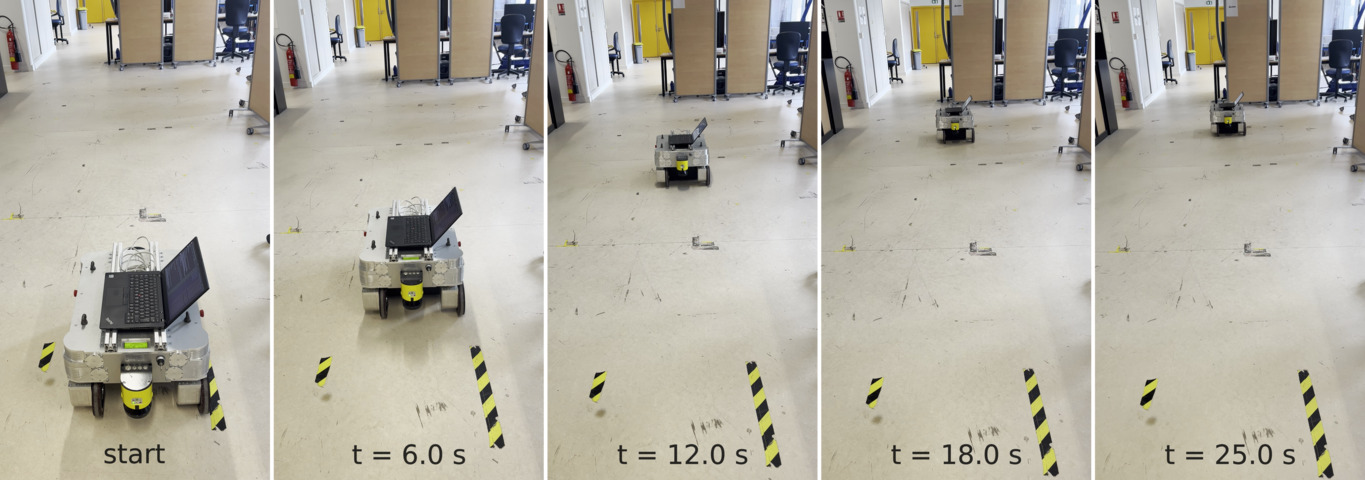
\includegraphics[width=\textwidth]{figures/SWMR/simulations/forward/snapshots.jpeg}
    \caption{Snapshots of the mobile base tracking a \textit{forward motion} trajectory.
        The robot accelerates for half the duration of the motion, eventually
        decelerating and stopping.}
    \label{fig:experiments:forward:snapshots}
\end{figure}
\begin{figure}
    \centering
    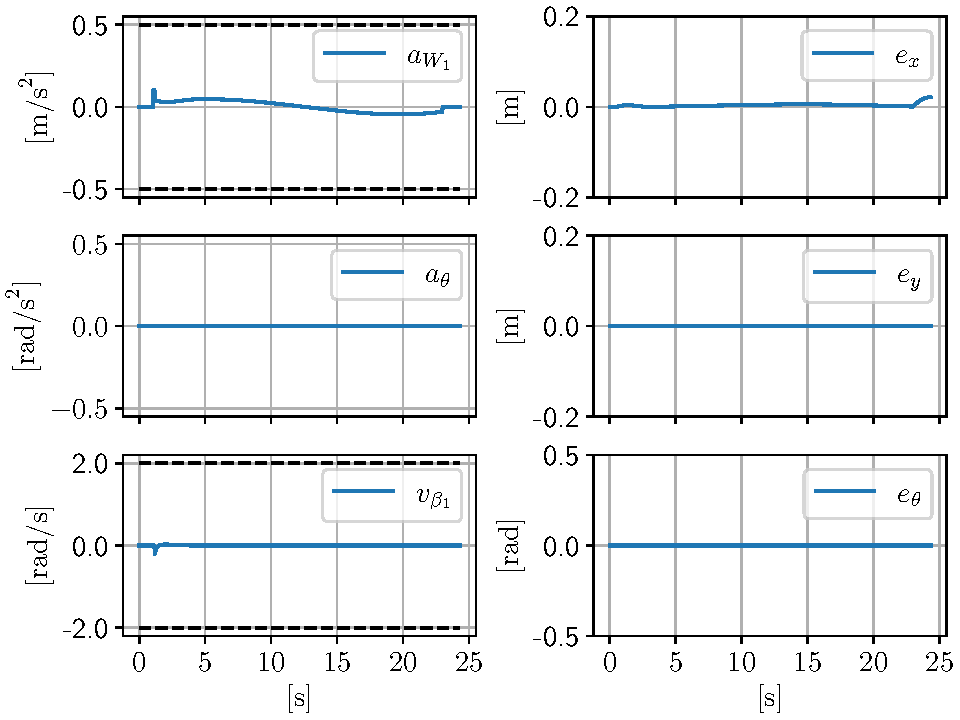
\includegraphics[width=0.75\textwidth]{figures/SWMR/simulations/forward/inputs_and_errors.pdf}
    \caption{Control inputs and trajectory tracking errors for the
        \textit{forward motion} trajectory.
    }
    \label{fig:simulations:forward:inputs-and-errors}
\end{figure}
\begin{figure}
    \centering
    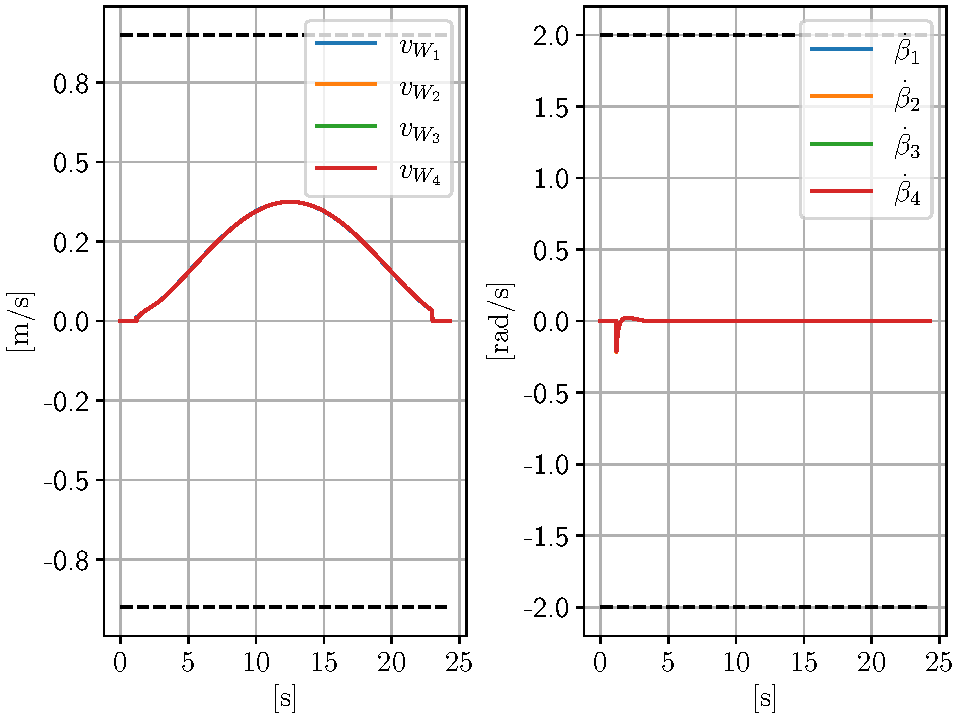
\includegraphics[width=0.75\textwidth]{figures/SWMR/simulations/forward/wheels_velocities.pdf}
    \caption{Driving and steering velocities of the four wheels for the
        \textit{forward motion} trajectory. The driving velocities are increasing
        for the first part of the motion, and decreasing until the robots stops
        for the second half. The steering velocities, apart for the first spike
        (due to numerical approximations), are always close to zero, indicating
        that the robot is not steering.}
    \label{fig:simulations:forward:wheel-velocities}
\end{figure}

The \textit{backward motion} trajectory is defined similarly to the
\textit{forward motion} trajectory, with the difference that
$v^{\mathrm{ref}}<0$. The initial orientation of the robot is $\theta_0=0.0$ [rad].
Moreover, $\beta_{1,0}=\beta_{2,0}=\beta_{3,0}=\beta_{4,0}=\pi$ [rad], $t_f = 25.0$
[s] and $v^{\mathrm{ref}}=0.2$ [m/s].
Figure \ref{fig:experiments:backward:snapshots}shows a sequence of snapshots of
the mobile base moving while tracking the considered trajectory.
Figure \ref{fig:simulations:backward:inputs-and-errors} show the control inputs
computed by the NMPC and the trajectory tracking error.
Figure \ref{fig:simulations:backward:wheel-velocities} shows the corresponding
driving and steering velocities. Note again, how constraints are always satisfied
during the motion of the robot. From the snapshots, it is possible to see that 
the robot is slightly deviating from the straight line. This behavior is due the 
odometric localization module, which is not as precise as a Kalman filter or
SLAM \cite{Thrun2005ProbabilisticRobotics}.
The integration of a better localization system will be part of future works.
\begin{figure}
    \centering
    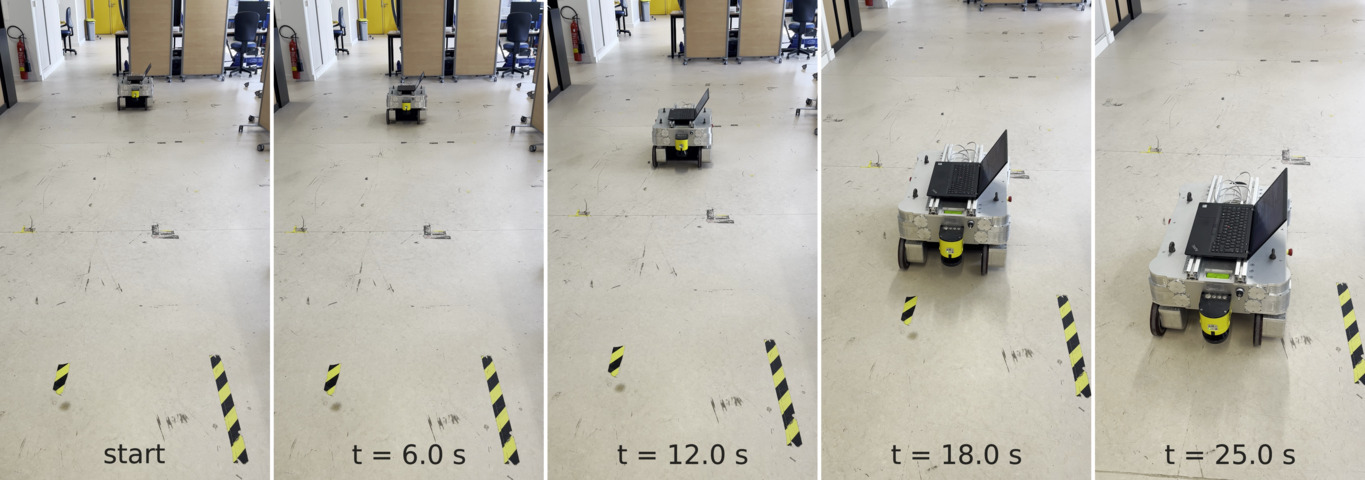
\includegraphics[width=\textwidth]{figures/SWMR/simulations/backward/snapshots.jpeg}
    \caption{Snapshots of the mobile base tracking a \textit{backward motion} trajectory.}
    \label{fig:experiments:backward:snapshots}
\end{figure}
\begin{figure}
    \centering
    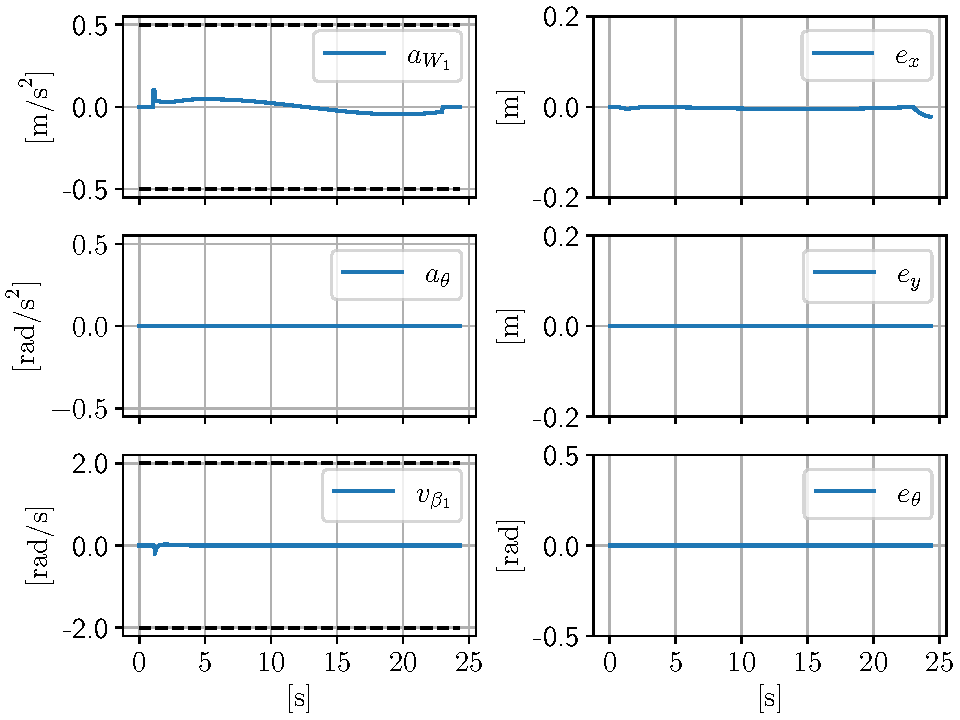
\includegraphics[width=0.75\textwidth]{figures/SWMR/simulations/backward/inputs_and_errors.pdf}
    \caption{Control inputs and trajectory tracking errors for the \textit{backward motion} trajectory.}
    \label{fig:simulations:backward:inputs-and-errors}
\end{figure}
\begin{figure}
    \centering
    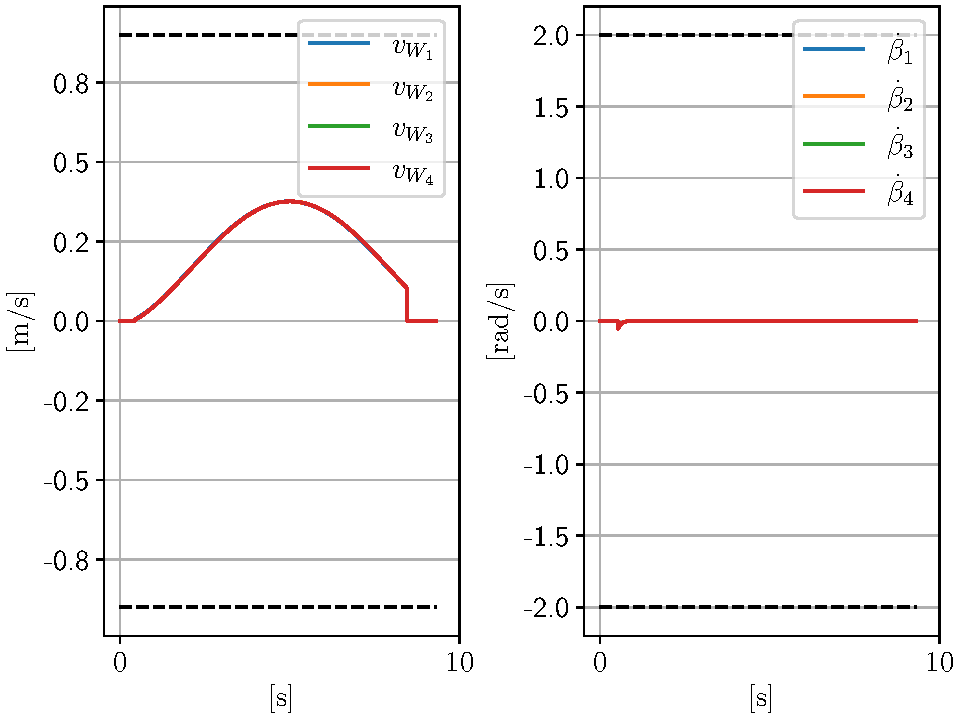
\includegraphics[width=0.75\textwidth]{figures/SWMR/simulations/backward/wheels_velocities.pdf}
    \caption{Driving and steering velocities of the four wheels for the \textit{backward motion} trajectory.}
    \label{fig:simulations:backward:wheel-velocities}
\end{figure}

The \textit{diagonal motion} trajectory is defined similarly to the
\textit{forward motion} trajectory, but with $\theta^{\mathrm{dir}} \ne \theta_0$.
The initial orientation of the robot is $\theta_0=\pi/4$ [rad].
Moreover, $\beta_{1,0}=\beta_{2,0}=\beta_{3,0}=\beta_{4,0}=-\pi/4$ [rad], $t_f = 25.0$
[s] and $v^{\mathrm{ref}}=0.2$ [m/s].
Figure \ref{fig:experiments:diagonal:snapshots} shows a sequence of snapshots of
the mobile base moving while tracking the considered trajectory.
Figure \ref{fig:simulations:diagonal:inputs-and-errors} show the control
inputs computed by the NMPC and the trajectory tracking error.
Figure \ref{fig:simulations:diagonal:wheel-velocities} shows the corresponding
driving and steering velocities. Once again, the trajectory is tracking while 
keeping the error close to zero, and satisfying all constraints of the system.
\begin{figure}
    \centering
    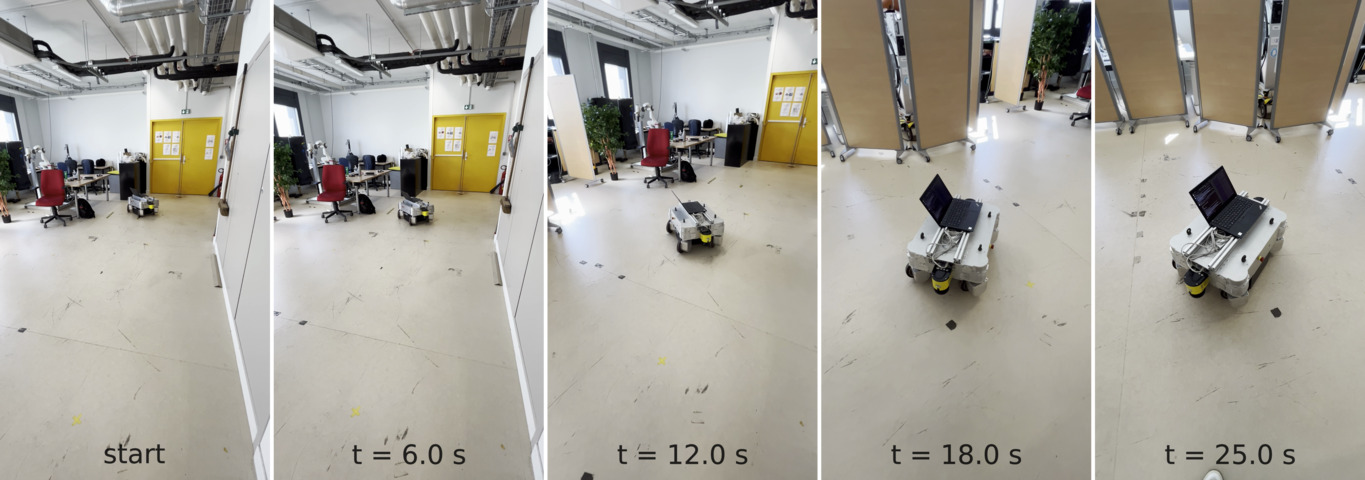
\includegraphics[width=\textwidth]{figures/SWMR/simulations/diagonal/snapshots.jpeg}
    \caption{Snapshots of the mobile base tracking a \textit{diagonal motion} trajectory.}
    \label{fig:experiments:diagonal:snapshots}
\end{figure}
\begin{figure}
    \centering
    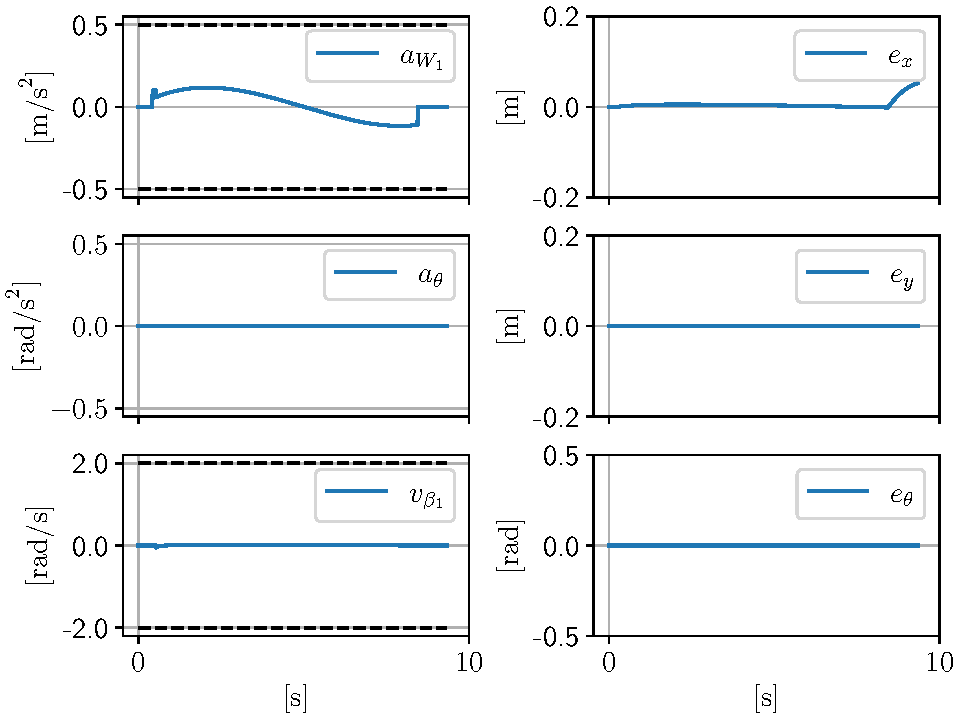
\includegraphics[width=0.75\textwidth]{figures/SWMR/simulations/diagonal/inputs_and_errors.pdf}
    \caption{Control inputs and trajectory tracking errors for the
        \textit{diagonal motion} trajectory.}
    \label{fig:simulations:diagonal:inputs-and-errors}
\end{figure}
\begin{figure}
    \centering
    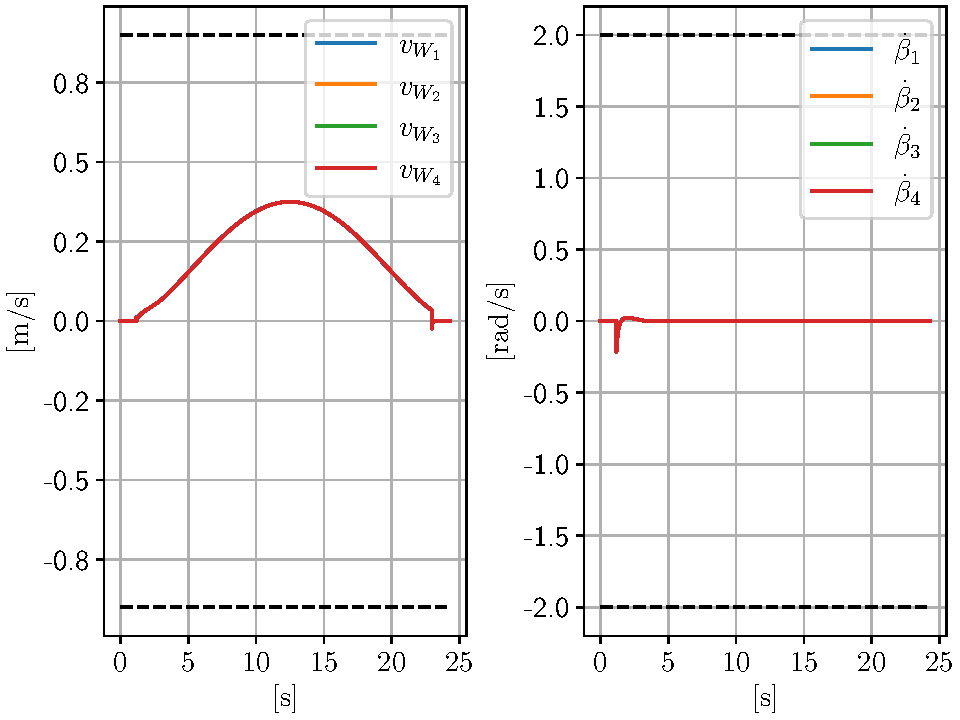
\includegraphics[width=0.75\textwidth]{figures/SWMR/simulations/diagonal/wheels_velocities.pdf}
    \caption{Driving and steering velocities of the four wheels for the
        \textit{diagonal motion} trajectory. The profile is similar to the 
        case of moving forward because the initial configuration of the steerable 
        joints are displaced by $\pi$ [rad] with respect to the previous 
        experiment.}
    \label{fig:simulations:diagonal:wheel-velocities}
\end{figure}

In all these experiments (\textit{forward}, \textit{backward} and
\textit{diagonal motion}), the reference position of the robot is the same.
The reference orientation, on the other hand, is different.
Note that the robot is able to track diagonal trajectories because of the
steerable wheels, which allow the mobile base behave as an omnidirectional robot.

\subsection{Circular motions}
In this section, we consider tasks in which the robot is required to follow
a circle with center $(x_C, y_C)$ and radius $R > 0$.
The reference position, which is in common among all circular trajectories
(defined below), is given by
\begin{subequations}
    \begin{align*}
        x^{\mathrm{ref}}(s) &= x_C + R \cos(\phi + 2 \pi s) \\
        y^{\mathrm{ref}}(s) &= y_C + R \sin(\phi + 2 \pi s).
    \end{align*} 
\end{subequations}

In the \textit{circle with constant orientation} trajectory,
the reference orientation is defined by
\begin{subequations}
\begin{align*}
    \theta^{\mathrm{ref}}(t) &= \theta_0,
\end{align*}
\end{subequations}
with $\theta_0=\pi$ [rad]. The initial configuration of the steering angles
are given by$\beta_{1,0}=\beta_{2,0}=\beta_{3,0}=\beta_{4,0}=0.0$ [rad].
Moreover, $R=0.5$ [m], $\phi=\pi/2$ [rad], and $t_f=15.7$~[s].

Similarly to the \textit{diagonal motion}, the robot is able to track a
circle while keeping its orientation constant because of the steerable wheels.
This kind of motion, indeed, would not be possible with a differential drive robot.
Figure \ref{fig:experiments:circle-with-constant-orientation:snapshots}
shows a sequence of snapshots of the mobile base moving while tracking the
considered trajectory.
Figure \ref{fig:simulations:circle-with-constant-orientation:inputs-and-errors}
shows the control inputs computed by the NMPC and the trajectory tracking error.
Figure \ref{fig:simulations:circle-with-constant-orientation:wheel-velocities}
shows the corresponding driving and steering velocities.
\begin{figure}
    \centering
    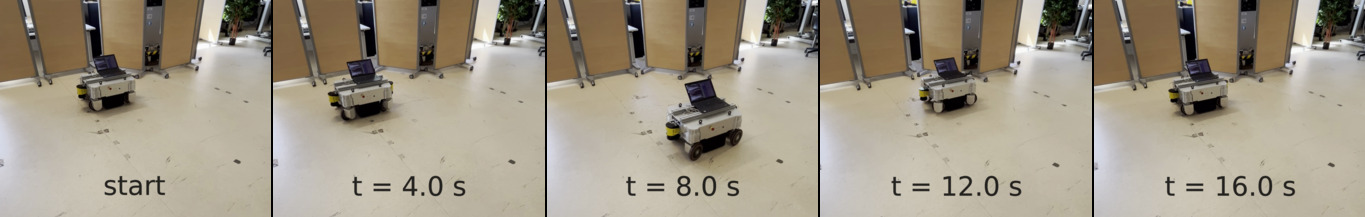
\includegraphics[width=\textwidth]{figures/SWMR/simulations/circular_with_constant_orientation/snapshots.jpeg}
    \caption{Snapshots of the mobile base tracking a
        \textit{circle with constant orientation}. Notice how the robot keeps 
        the same orientation throughout the motion. This is possible because 
        of the omnidirectional capabilities of the platform.}
    \label{fig:experiments:circle-with-constant-orientation:snapshots}
\end{figure}
\begin{figure}
    \centering
    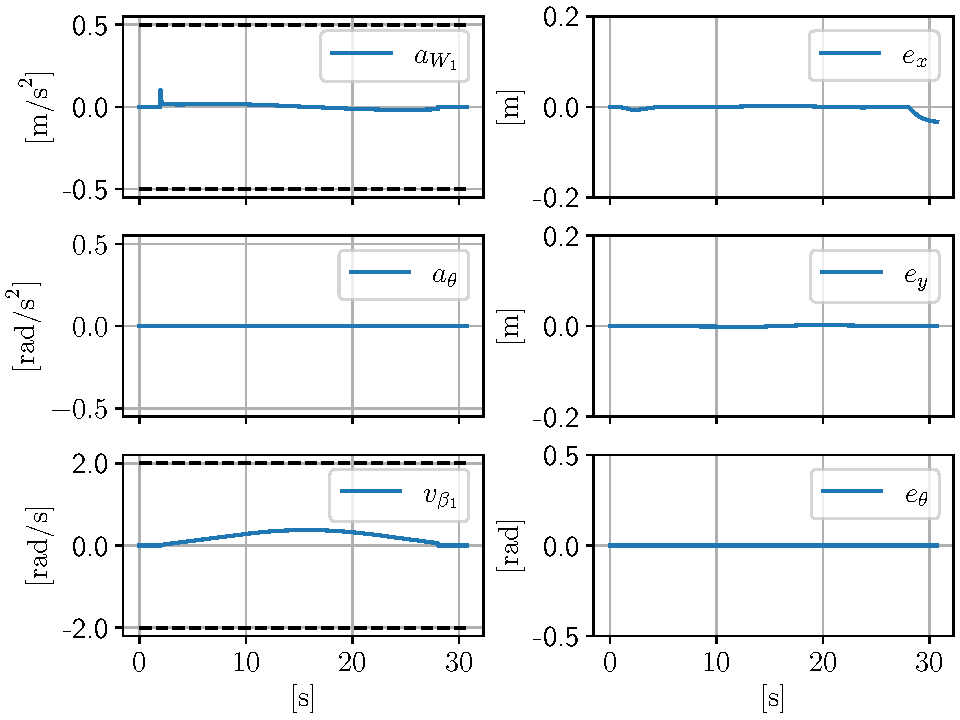
\includegraphics[width=0.8\textwidth]{figures/SWMR/simulations/circular_with_constant_orientation/inputs_and_errors.pdf}
    \caption{Control inputs and trajectory tracking errors for the \textit{circle with constant orientation} trajectory.}
    \label{fig:simulations:circle-with-constant-orientation:inputs-and-errors}
\end{figure}
\begin{figure}
    \centering
    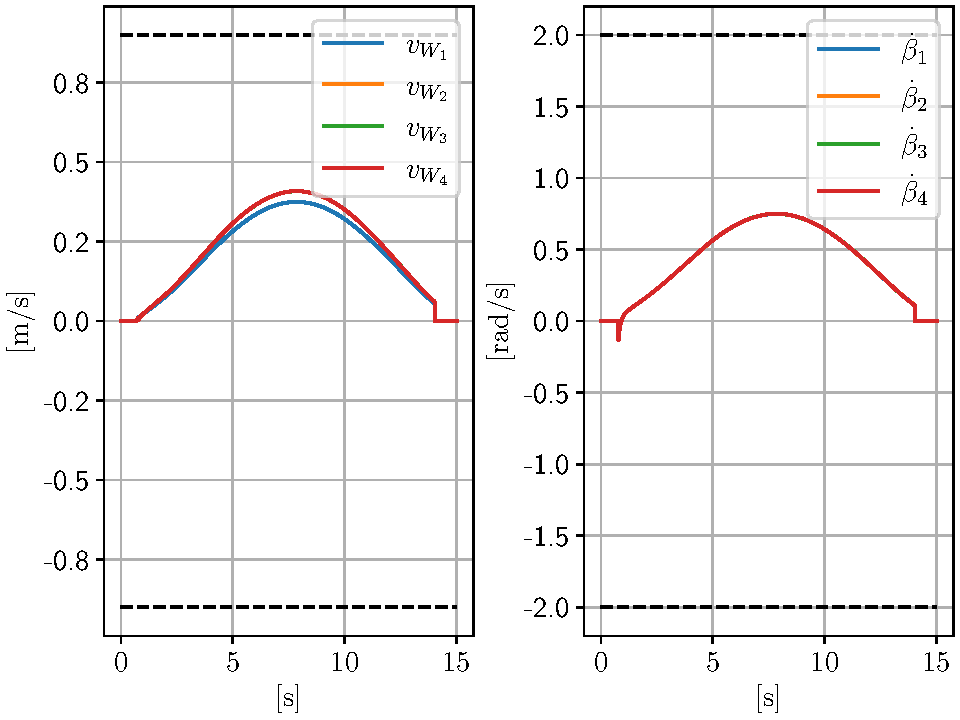
\includegraphics[width=0.8\textwidth]{figures/SWMR/simulations/circular_with_constant_orientation/wheels_velocities.pdf}
    \caption{Driving and steering velocities of the four wheels for the \textit{circle with constant orientation} trajectory.}
    \label{fig:simulations:circle-with-constant-orientation:wheel-velocities}
\end{figure}

In the \textit{circle with tangent orientation} trajectory, the reference
orientation is defined by
\begin{equation}
    \theta^{\mathrm{ref}}(s) = \mathrm{atan2}\left(\frac{\partial y^{\mathrm{ref}}(s)}{\partial s}, \frac{\partial x^{\mathrm{ref}}(s)}{\partial s}\right).
    \label{eq:reference-tangent-orientation}
\end{equation}
with $\theta_0=\pi$ [rad], $\beta_{1,0}=\beta_{2,0}=\beta_{3,0}=\beta_{4,0}=0.0$ [rad].
Moreover, $R=0.5$ [m], $\phi=\pi/2$ [rad], and $t_f=15.7$~[s].
Figure \ref{fig:experiments:circle-with-tangent-orientation:snapshots} shows
a sequence of snapshots of the robot moving while tracking this trajectory.
Here, it is possible to notice how the mobile base changes its orientation
according to the previously defined circle, ending up in its initial pose at
the end of the motion.
Figure \ref{fig:simulations:circle-with-tangent-orientation:inputs-and-errors}
show the control inputs computed by the NMPC, together with the trajectory
tracking error.
Figure \ref{fig:simulations:circle-with-tangent-orientation:wheel-velocities}
shows the corresponding driving and steering velocities.
The trajectory tracking error is always close to zero, and the control inputs,
together with steering and driving velocities of the wheels, are always within
their boundaries.
\begin{figure}
    \centering
    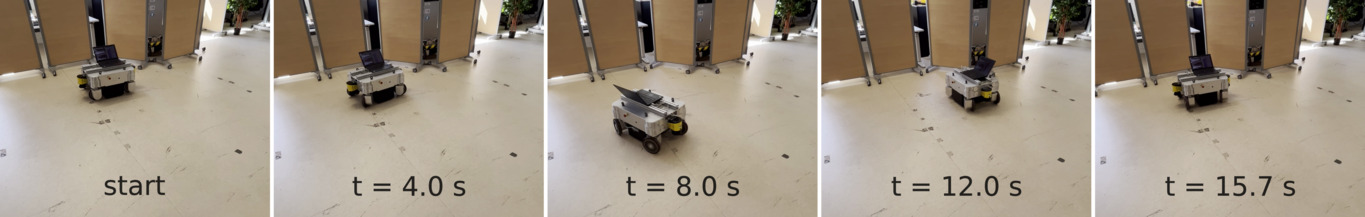
\includegraphics[width=\textwidth]{figures/SWMR/simulations/circular_with_tangent_orientation/snapshots.jpeg}
    \caption{Snapshots of the mobile robot tracking a \textit{circle with tangent orientation}.}
    \label{fig:experiments:circle-with-tangent-orientation:snapshots}
\end{figure}
\begin{figure}
    \centering
    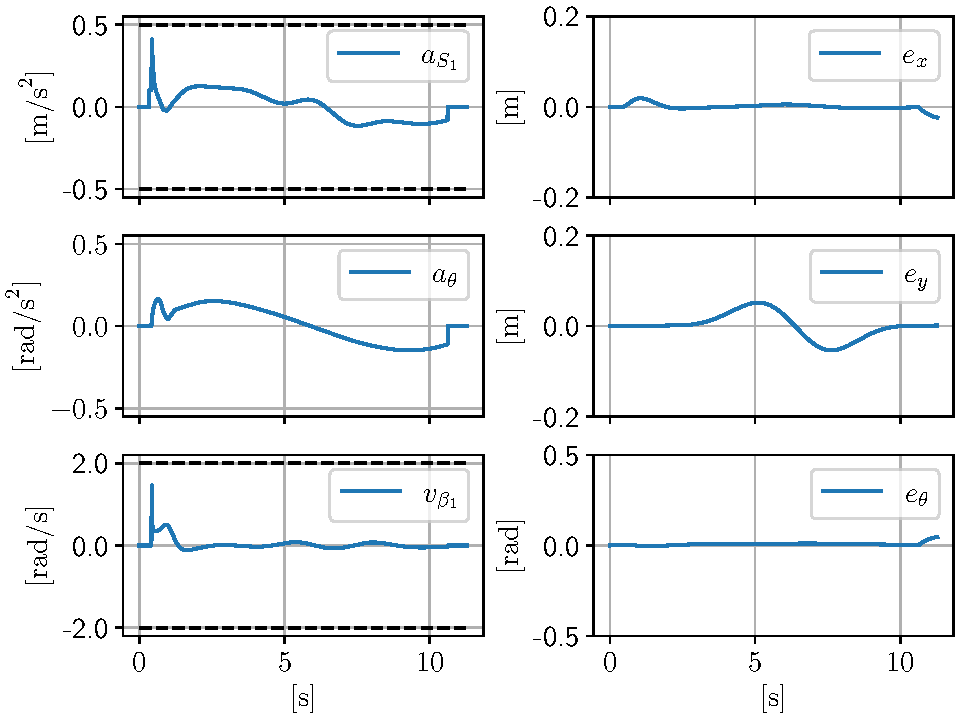
\includegraphics[width=0.75\textwidth]{figures/SWMR/simulations/circular_with_tangent_orientation/inputs_and_errors.pdf}
    \caption{Control inputs and trajectory tracking errors for the \textit{circle with tangent orientation} trajectory.}
    \label{fig:simulations:circle-with-tangent-orientation:inputs-and-errors}
\end{figure}
\begin{figure}
    \centering
    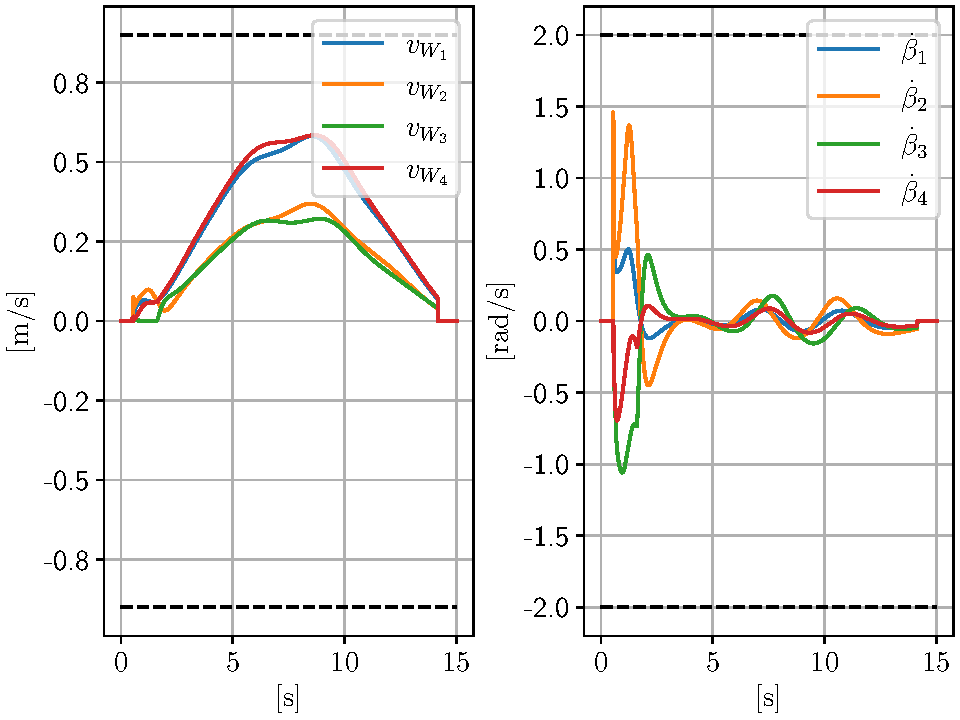
\includegraphics[width=0.75\textwidth]{figures/SWMR/simulations/circular_with_tangent_orientation/wheels_velocities.pdf}
    \caption{Driving and steering velocities of the four wheels for the \textit{circle with tangent orientation} trajectory.}
    \label{fig:simulations:circle-with-tangent-orientation:wheel-velocities}
\end{figure}

In the \textit{circle with inward orientation} trajectory, the robot is required
to follow the previously defined circle, while pointing its front towards
the center of the circle itself. The reference orientation is defined as
\begin{subequations}
\begin{align*}
    \theta^{\mathrm{ref}}(s) &= \mathrm{atan2}(y_C - y^{\mathrm{ref}}(s), x_C - x^{\mathrm{ref}}(s)).
\end{align*}
\end{subequations}
Here, $\theta_0=-\pi/2$ [rad], $\beta_{1,0}=\beta_{2,0}=\beta_{3,0}=\beta_{4,0}=-\pi/2$
[rad]. Moreover, $R=0.6$ [m], $\phi=\pi/2$ [rad], and $t_f=18.8$~[s].
Figure \ref{fig:experiments:circle-with-inward-orientation:snapshots} shows a
sequence of snapshots of the mobile base moving while tracking the reference
trajectory. In this experiment, it is possible to notice that the position of
the mobile base is identical to the one of the previous section.
The reference orientation, on the other hand, is such that the front of the
robot points towards the center of the circle.
Figure \ref{fig:simulations:circle-with-inward-orientation:inputs-and-errors}
shows the control inputs computed by the NMPC and the trajectory tracking error.
Figure \ref{fig:simulations:circle-with-inward-orientation:wheel-velocities}
shows the corresponding driving and steering velocities. 
\begin{figure}
    \centering
    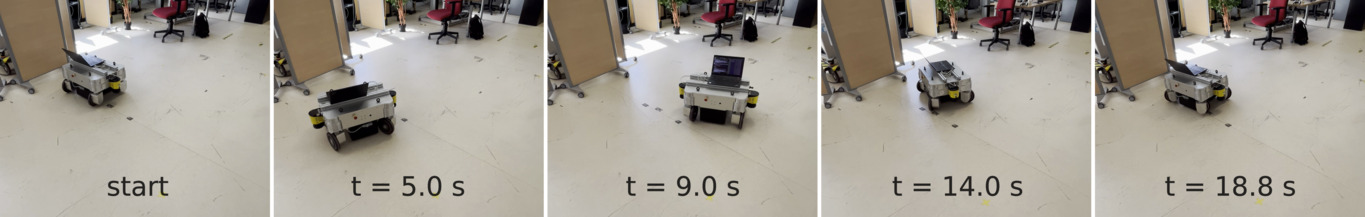
\includegraphics[width=\textwidth]{figures/SWMR/simulations/circular_with_inward_orientation/snapshots.jpeg}
    \caption{Snapshots of the mobile base tracking a \textit{circle with inward orientation}.}
    \label{fig:experiments:circle-with-inward-orientation:snapshots}
\end{figure}
\begin{figure}
    \centering
    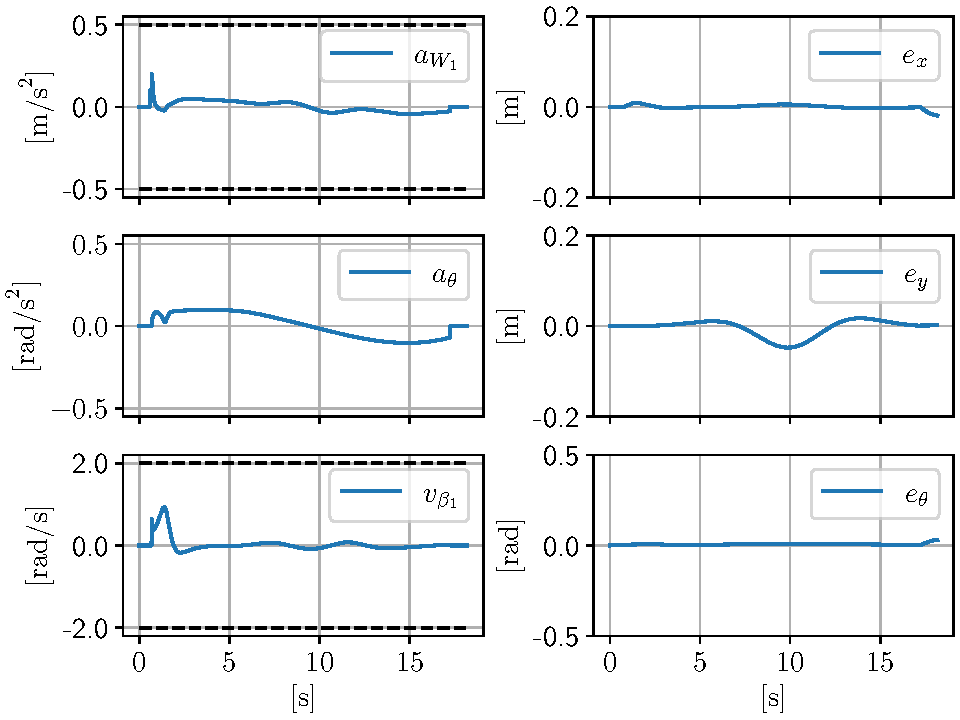
\includegraphics[width=0.75\textwidth]{figures/SWMR/simulations/circular_with_inward_orientation/inputs_and_errors.pdf}
    \caption{Control inputs and trajectory tracking errors for the \textit{circle with inward orientation} trajectory.}
    \label{fig:simulations:circle-with-inward-orientation:inputs-and-errors}
\end{figure}
\begin{figure}
    \centering
    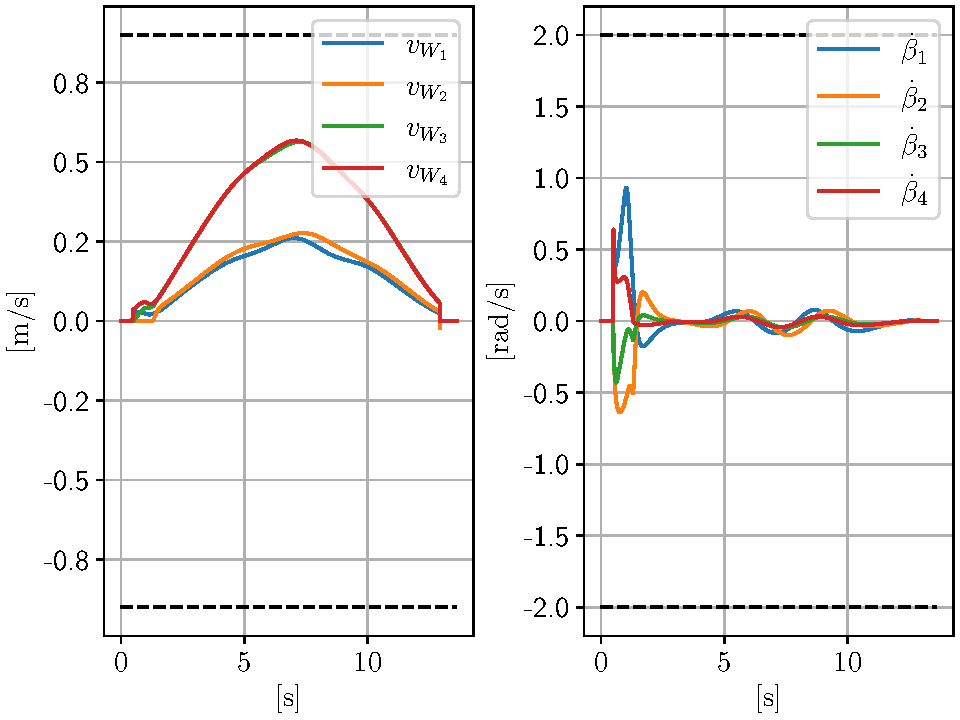
\includegraphics[width=0.75\textwidth]{figures/SWMR/simulations/circular_with_inward_orientation/wheels_velocities.pdf}
    \caption{Driving and steering velocities of the four wheels for the \textit{circle with inward orientation} trajectory.}
    \label{fig:simulations:circle-with-inward-orientation:wheel-velocities}
\end{figure}

In the \textit{circle with outward orientation} trajectory, the robot is
required to follow the previously defined circle, while pointing its back
towards the center of the circle itself. The reference orientation is defined as
\begin{subequations}
\begin{align*}
    \theta^{\mathrm{ref}}(s) &= \mathrm{atan2}(y^{\mathrm{ref}}(s) - y_C, x^{\mathrm{ref}}(s) - x_C).
\end{align*}
\end{subequations}
Here, $\theta_0=\pi/2$ [rad], $\beta_{1,0}=\beta_{2,0}=\beta_{3,0}=\beta_{4,0}=\pi/2$
[rad]. Moreover, $R=0.6$ [m], $\phi=\pi/2$ [rad], and $t_f=18.8$~[s].
Figure \ref{fig:experiments:circle-with-outward-orientation:snapshots} shows
a sequence of snapshots of the mobile base moving while tracking the
considered trajectory.
Figure \ref{fig:simulations:circle-with-outward-orientation:inputs-and-errors}
show the control inputs computed by the NMPC and the trajectory tracking error.
Figure \ref{fig:simulations:circle-with-outward-orientation:wheel-velocities}
shows the corresponding driving and steering velocities. In this experiment,
the behavior is similar to the \textit{circle with inward orientation}, as the 
only difference in the reference trajectory is the orientation of the base.
\begin{figure}
    \centering
    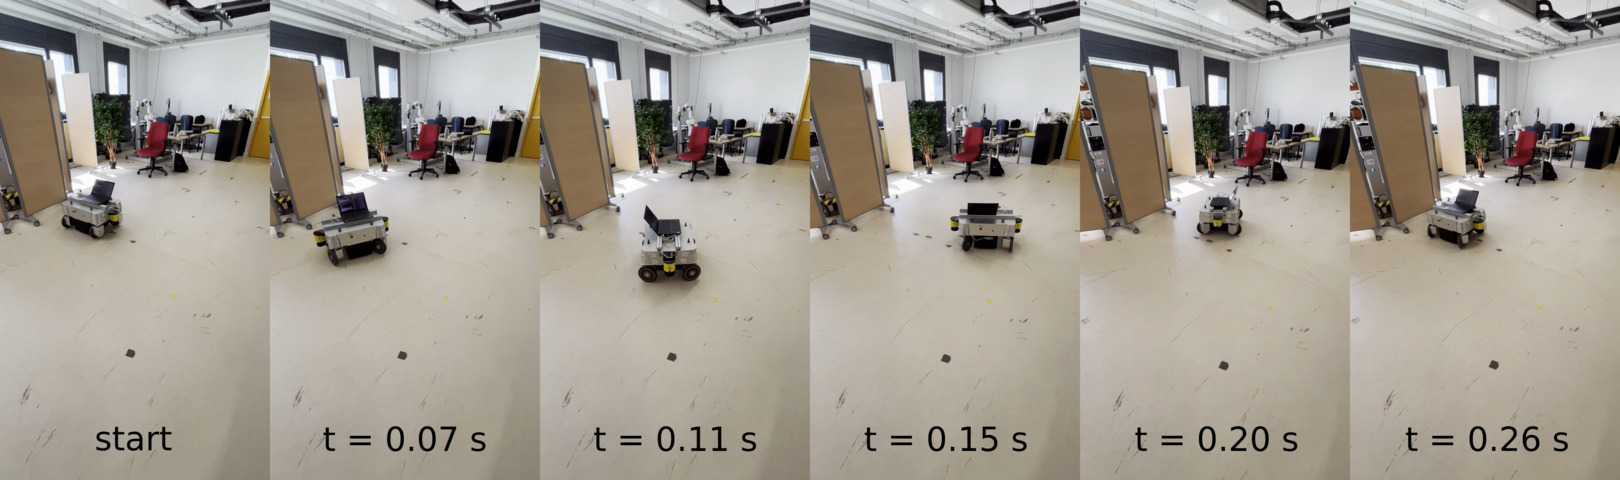
\includegraphics[width=\textwidth]{figures/SWMR/simulations/circular_with_outward_orientation/snapshots.jpeg}
    \caption{Snapshots of the mobile base tracking a \textit{circle with outward orientation}.}
    \label{fig:experiments:circle-with-outward-orientation:snapshots}
\end{figure}
\begin{figure}
    \centering
    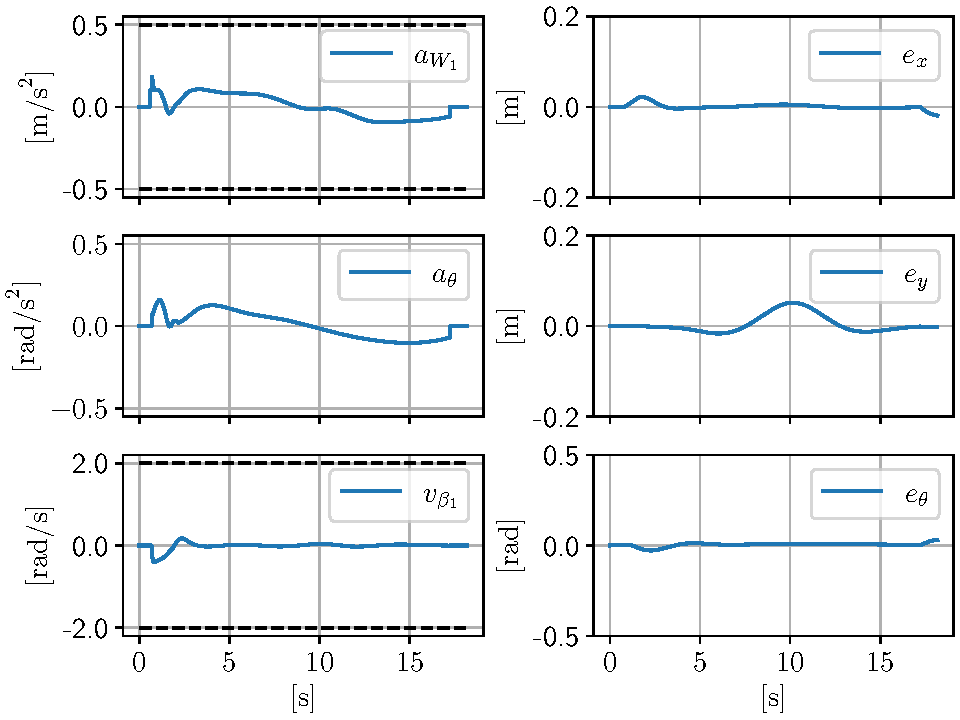
\includegraphics[width=0.8\textwidth]{figures/SWMR/simulations/circular_with_outward_orientation/inputs_and_errors.pdf}
    \caption{Control inputs and trajectory tracking errors for the \textit{circle with outward orientation} trajectory.}
    \label{fig:simulations:circle-with-outward-orientation:inputs-and-errors}
\end{figure}
\begin{figure}
    \centering
    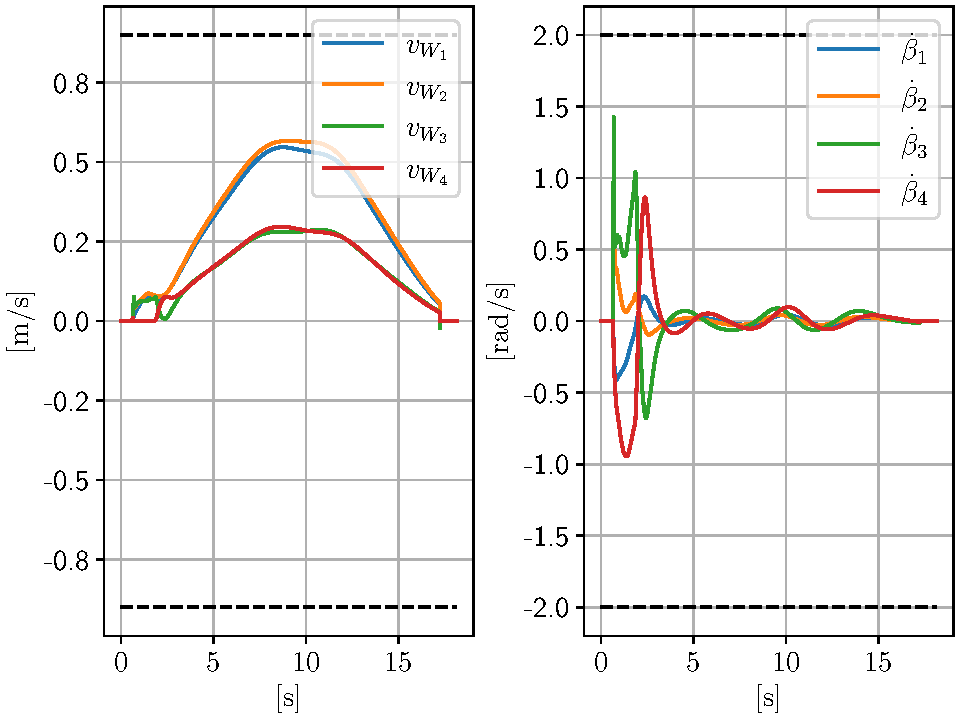
\includegraphics[width=0.8\textwidth]{figures/SWMR/simulations/circular_with_outward_orientation/wheels_velocities.pdf}
    \caption{Driving and steering velocities of the four wheels for the \textit{circle with outward orientation} trajectory.}
    \label{fig:simulations:circle-with-outward-orientation:wheel-velocities}
\end{figure}

\subsection{Slalom motions}
In this section, we consider tasks in which the robot is required to follow
a sinusoidal trajectory. The reference position, which is in common among all
trajectories defined below, is given by
\begin{subequations}
\begin{align*}
    x^{\mathrm{ref}}(s) &= 2 \pi s \\
    y^{\mathrm{ref}}(s) &= \alpha \sin(2 \pi s).
\end{align*}
\end{subequations}

In the \textit{slalom with constant orientation} trajectory, the robot is
required to follow the above defined sinusoidal trajectory while keeping its
orientation constant. The reference orientation is given by
\begin{subequations}
\begin{align*}
    \theta^{\mathrm{ref}}(t) &= \theta_0.
\end{align*}
\end{subequations}
Here, the initial orientation of the robot is $\theta_0=0.0$ [rad].
Moreover, $\beta_{1,0}=\beta_{2,0}=\beta_{3,0}=\beta_{4,0}=0.0$ [rad],
$\alpha=0.8$, and $t_f=31.4$~[s].

Note that, similarly to the \textit{circle with tangent orientation},
the tracking of this kind of trajectory is only possible because of the
steerable wheels.
Figure \ref{fig:experiments:slalom-with-constant-orientation:snapshots} shows
a sequence of snapshots of the mobile base moving while tracking the considered
trajectory.
Figure \ref{fig:simulations:slalom-with-constant-orientation:inputs-and-errors}
show the control inputs computed by the NMPC and the trajectory tracking error.
Figure \ref{fig:simulations:slalom-with-constant-orientation:wheel-velocities} 
shows the corresponding driving and steering velocities. Note that the spike 
in the steering velocities computed by the NMPC is due to the initial 
configuration of the wheels, which are not aligned with respect to the 
reference trajectory the robot is required to track.
In this case, the state trajectory generation scheme 
generates a state trajectory of the steering velocities which do not 
satisfy the constraints of the platform. The NMPC is able to take this into 
account, generating a control action which satisfy all requirements. The
resulting behavior is a realignment of the steerable wheels at the beginning of 
the motion, which makes it possible to successfully complete the assigned task.
\begin{figure}
    \centering
    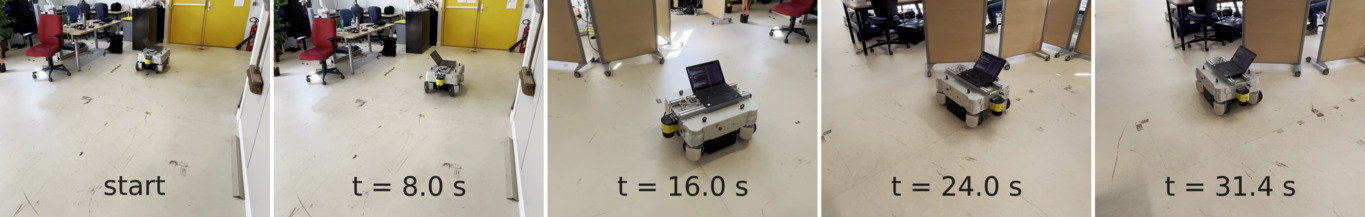
\includegraphics[width=\textwidth]{figures/SWMR/simulations/slalom_with_constant_orientation/snapshots.jpeg}
    \caption{Snapshots of the mobile base tracking a
        \textit{slalom with constant orientation}. Notice how the robot keeps 
        the same orientation throughout the motion. Again, this behavior
        is possible because of the omnidirectional capabilities of the platform.
    }
    \label{fig:experiments:slalom-with-constant-orientation:snapshots}
\end{figure}
\begin{figure}
    \centering
    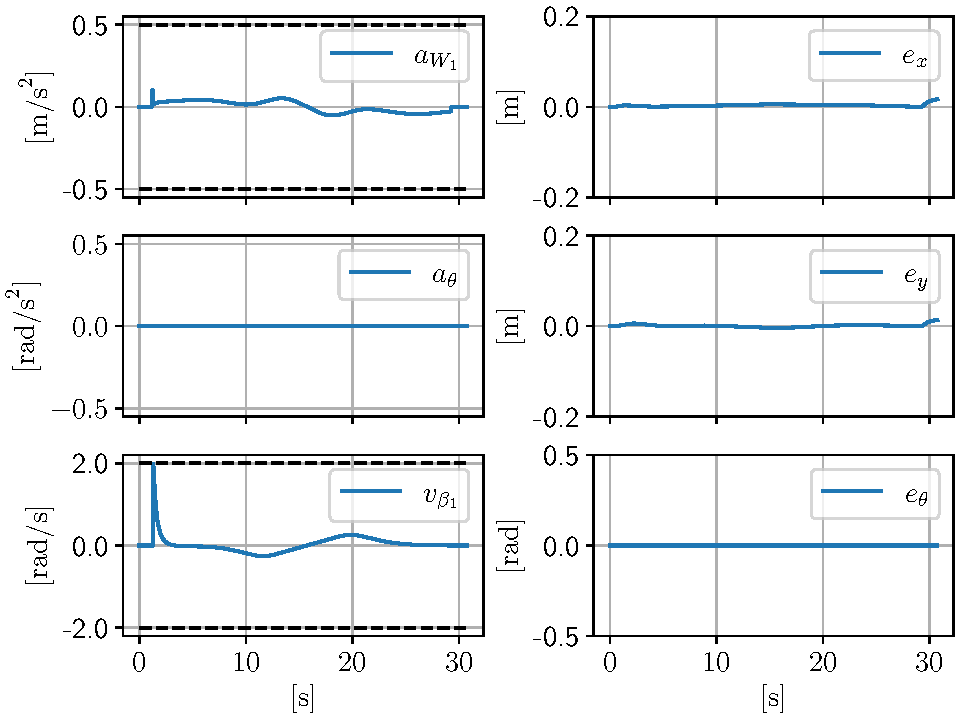
\includegraphics[width=0.8\textwidth]{figures/SWMR/simulations/slalom_with_constant_orientation/inputs_and_errors.pdf}
    \caption{Control inputs and trajectory tracking errors for the
        \textit{slalom with constant orientation} trajectory. Notice how 
        the steering velocity $v_{\beta_1}$ is at the upper bound when 
        the FSM changes its state from \textit{Starting} to \textit{Moving}.
        This is because of the state trajectory generation scheme, which 
        generates too high velocities, because of the steerable wheels which
        are not aligned with the reference trajectory at the beginning of 
        the motion. The NMPC is capable of taking this into account, generating
        feasible control inputs.
    }
    \label{fig:simulations:slalom-with-constant-orientation:inputs-and-errors}
\end{figure}
\begin{figure}
    \centering
    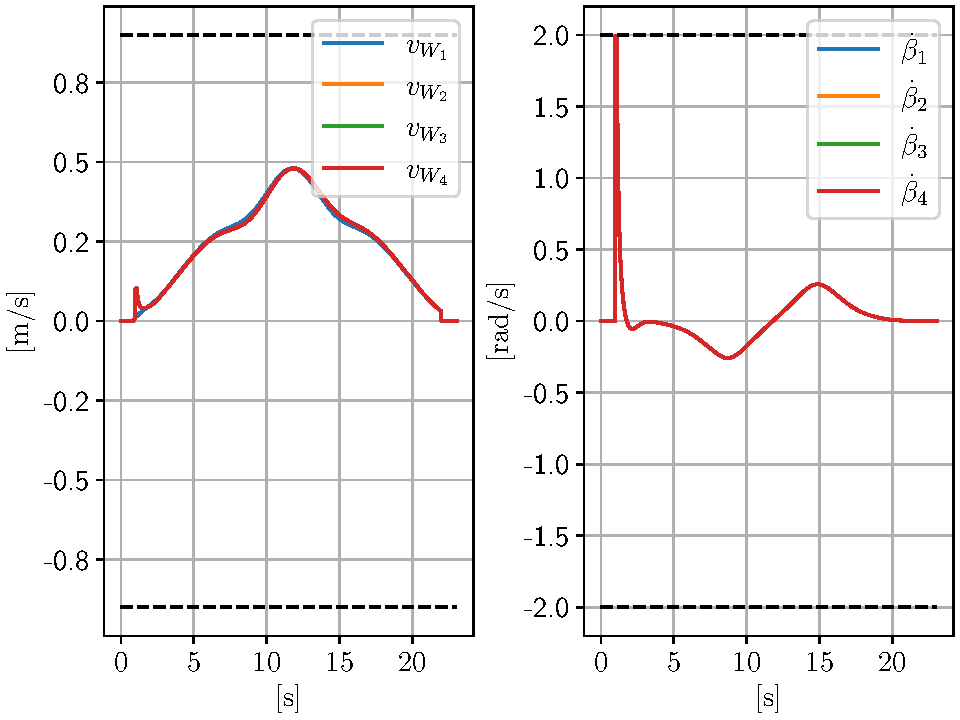
\includegraphics[width=0.8\textwidth]{figures/SWMR/simulations/slalom_with_constant_orientation/wheels_velocities.pdf}
    \caption{Driving and steering velocities of the four wheels for the
        \textit{slalom with constant orientation} trajectory. The steering 
        velocities at the limit of the bound at the beginning of the motion 
        reflect the behavior of the control inputs computed by the NMPC.
    }
    \label{fig:simulations:slalom-with-constant-orientation:wheel-velocities}
\end{figure}

In the \textit{slalom with tangent orientation} trajectory, the robot is
required to follow again the sinusoidal trajectory defined above, but while
keeping its orientation tangent to the trajectory itself.
The reference orientation is given by eq. \eqref{eq:reference-tangent-orientation}.
Here, the initial orientation of the robot is $\theta_0=\mathrm{atan}(\alpha)$
[rad]. Moreover, $\beta_{1,0}=\beta_{2,0}=\beta_{3,0}=\beta_{4,0}=0.0$ [rad],
with $\alpha=0.8$, and $t_f=31.4$~[s].

Figure \ref{fig:experiments:slalom-with-tangent-orientation:snapshots} shows
a sequence of snapshots of the mobile base moving while tracking the
considered trajectory. Here, the reference position is the same as the one
defined in the previous section, while the reference orientation in different.
In the snapshots, it is possible to notice how the robot tracks the slalom
while keeping its orientation tangent to the slalom itself.
Figure \ref{fig:simulations:slalom-with-tangent-orientation:inputs-and-errors}
shows the control inputs computed by the NMPC and the trajectory tracking error,
which is always close to zero.
Figure \ref{fig:simulations:slalom-with-tangent-orientation:wheel-velocities}
shows the corresponding driving and steering velocities.
Once again, the NMPC generates feasible control inputs while satisfying driving
and steering velocity constraints on all wheels.
\begin{figure}
    \centering
    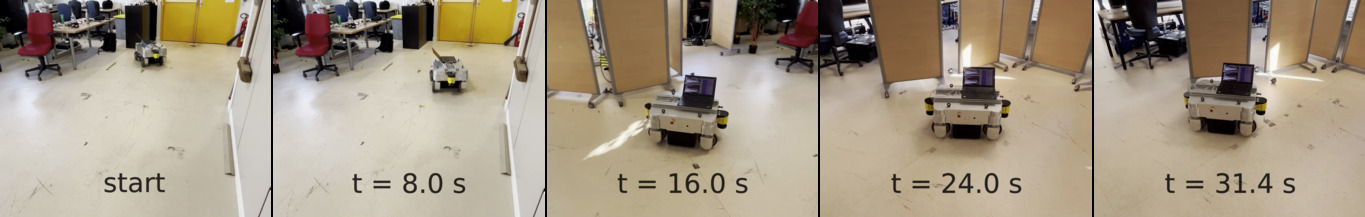
\includegraphics[width=\textwidth]{figures/SWMR/simulations/slalom_with_tangent_orientation/snapshots.jpeg}
    \caption{Snapshots of the mobile base tracking a \textit{slalom with tangent orientation}.}
    \label{fig:experiments:slalom-with-tangent-orientation:snapshots}
\end{figure}
\begin{figure}
    \centering
    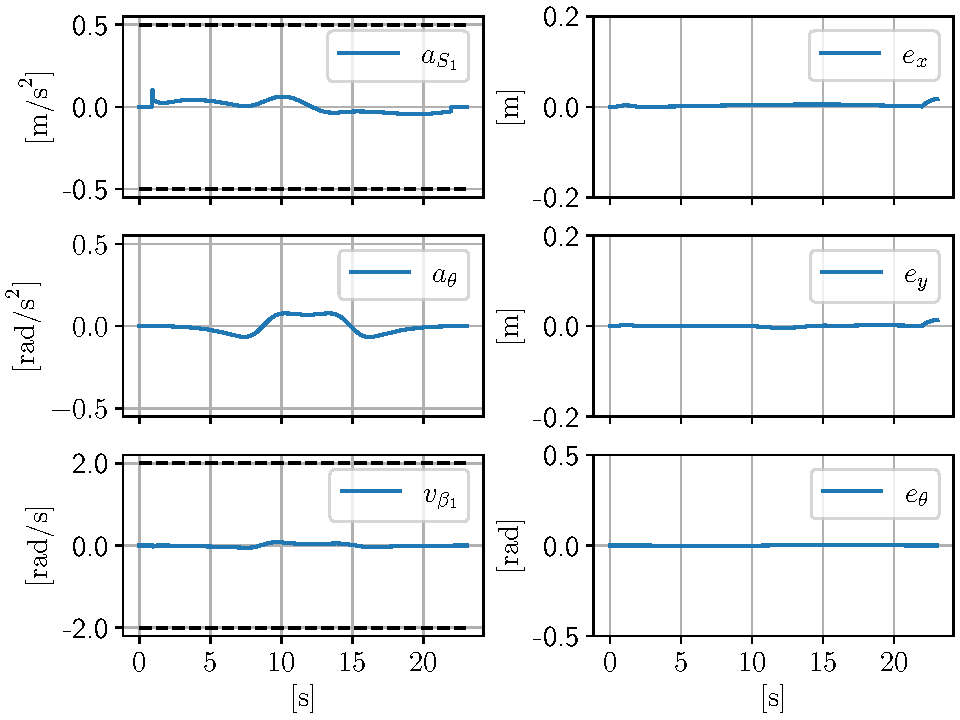
\includegraphics[width=0.75\textwidth]{figures/SWMR/simulations/slalom_with_tangent_orientation/inputs_and_errors.pdf}
    \caption{Control inputs and trajectory tracking errors for the
        \textit{slalom with tangent orientation} trajectory.
    }
    \label{fig:simulations:slalom-with-tangent-orientation:inputs-and-errors}
\end{figure}
\begin{figure}
    \centering
    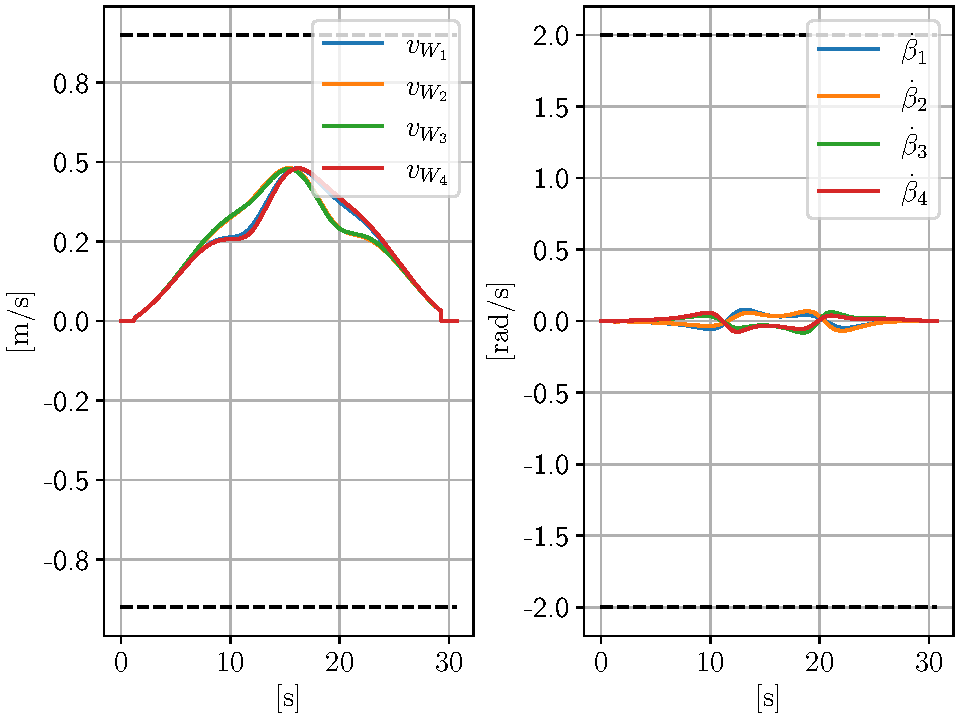
\includegraphics[width=0.75\textwidth]{figures/SWMR/simulations/slalom_with_tangent_orientation/wheels_velocities.pdf}
    \caption{Driving and steering velocities of the four wheels for the
        \textit{slalom with tangent orientation} trajectory.
    }
    \label{fig:simulations:slalom-with-tangent-orientation:wheel-velocities}
\end{figure}
